\documentclass[twoside]{book}

% Packages required by doxygen
\usepackage{calc}
\usepackage{doxygen}
\usepackage{graphicx}
\usepackage[utf8]{inputenc}
\usepackage{makeidx}
\usepackage{multicol}
\usepackage{multirow}
\usepackage{textcomp}
\usepackage[table]{xcolor}

% Font selection
\usepackage[T1]{fontenc}
\usepackage{mathptmx}
\usepackage[scaled=.90]{helvet}
\usepackage{courier}
\usepackage{amssymb}
\usepackage{sectsty}
\renewcommand{\familydefault}{\sfdefault}
\allsectionsfont{%
  \fontseries{bc}\selectfont%
  \color{darkgray}%
}
\renewcommand{\DoxyLabelFont}{%
  \fontseries{bc}\selectfont%
  \color{darkgray}%
}

% Page & text layout
\usepackage{geometry}
\geometry{%
  a4paper,%
  top=2.5cm,%
  bottom=2.5cm,%
  left=2.5cm,%
  right=2.5cm%
}
\tolerance=750
\hfuzz=15pt
\hbadness=750
\setlength{\emergencystretch}{15pt}
\setlength{\parindent}{0cm}
\setlength{\parskip}{0.2cm}
\makeatletter
\renewcommand{\paragraph}{%
  \@startsection{paragraph}{4}{0ex}{-1.0ex}{1.0ex}{%
    \normalfont\normalsize\bfseries\SS@parafont%
  }%
}
\renewcommand{\subparagraph}{%
  \@startsection{subparagraph}{5}{0ex}{-1.0ex}{1.0ex}{%
    \normalfont\normalsize\bfseries\SS@subparafont%
  }%
}
\makeatother

% Headers & footers
\usepackage{fancyhdr}
\pagestyle{fancyplain}
\fancyhead[LE]{\fancyplain{}{\bfseries\thepage}}
\fancyhead[CE]{\fancyplain{}{}}
\fancyhead[RE]{\fancyplain{}{\bfseries\leftmark}}
\fancyhead[LO]{\fancyplain{}{\bfseries\rightmark}}
\fancyhead[CO]{\fancyplain{}{}}
\fancyhead[RO]{\fancyplain{}{\bfseries\thepage}}
\fancyfoot[LE]{\fancyplain{}{}}
\fancyfoot[CE]{\fancyplain{}{}}
\fancyfoot[RE]{\fancyplain{}{\bfseries\scriptsize Generated on Fri Apr 11 2014 18\-:11\-:48 for Sound Editor by Doxygen }}
\fancyfoot[LO]{\fancyplain{}{\bfseries\scriptsize Generated on Fri Apr 11 2014 18\-:11\-:48 for Sound Editor by Doxygen }}
\fancyfoot[CO]{\fancyplain{}{}}
\fancyfoot[RO]{\fancyplain{}{}}
\renewcommand{\footrulewidth}{0.4pt}
\renewcommand{\chaptermark}[1]{%
  \markboth{#1}{}%
}
\renewcommand{\sectionmark}[1]{%
  \markright{\thesection\ #1}%
}

% Indices & bibliography
\usepackage{natbib}
\usepackage[titles]{tocloft}
\setcounter{tocdepth}{3}
\setcounter{secnumdepth}{5}
\makeindex

% Hyperlinks (required, but should be loaded last)
\usepackage{ifpdf}
\ifpdf
  \usepackage[pdftex,pagebackref=true]{hyperref}
\else
  \usepackage[ps2pdf,pagebackref=true]{hyperref}
\fi
\hypersetup{%
  colorlinks=true,%
  linkcolor=blue,%
  citecolor=blue,%
  unicode%
}

% Custom commands
\newcommand{\clearemptydoublepage}{%
  \newpage{\pagestyle{empty}\cleardoublepage}%
}


%===== C O N T E N T S =====

\begin{document}

% Titlepage & ToC
\hypersetup{pageanchor=false}
\pagenumbering{roman}
\begin{titlepage}
\vspace*{7cm}
\begin{center}%
{\Large Sound Editor }\\
\vspace*{1cm}
{\large Generated by Doxygen 1.8.6}\\
\vspace*{0.5cm}
{\small Fri Apr 11 2014 18:11:48}\\
\end{center}
\end{titlepage}
\clearemptydoublepage
\tableofcontents
\clearemptydoublepage
\pagenumbering{arabic}
\hypersetup{pageanchor=true}

%--- Begin generated contents ---
\chapter{Hierarchical Index}
\section{Class Hierarchy}
This inheritance list is sorted roughly, but not completely, alphabetically\-:\begin{DoxyCompactList}
\item $<$A\-V\-Audio\-Player\-Delegate$>$\begin{DoxyCompactList}
\item \contentsline{section}{S\-E\-Sound()}{\pageref{category_s_e_sound_07_08}}{}
\end{DoxyCompactList}
\item $<$A\-V\-Audio\-Recorder\-Delegate$>$\begin{DoxyCompactList}
\item \contentsline{section}{S\-E\-Sound()}{\pageref{category_s_e_sound_07_08}}{}
\end{DoxyCompactList}
\item N\-S\-Object\begin{DoxyCompactList}
\item \contentsline{section}{S\-E\-Audio\-Stream}{\pageref{interface_s_e_audio_stream}}{}
\item \contentsline{section}{S\-E\-Audio\-Stream\-Player}{\pageref{interface_s_e_audio_stream_player}}{}
\item \contentsline{section}{S\-E\-Sound}{\pageref{interface_s_e_sound}}{}
\item \contentsline{section}{S\-R\-Audio\-Stream\-Player}{\pageref{interface_s_r_audio_stream_player}}{}
\end{DoxyCompactList}
\item $<$N\-S\-Object\-N\-S\-Object$>$\begin{DoxyCompactList}
\item \contentsline{section}{$<$S\-E\-Audio\-Stream\-Player\-Delegate$>$}{\pageref{protocol_s_e_audio_stream_player_delegate-p}}{}
\item \contentsline{section}{$<$S\-R\-Audio\-Stream\-Delegate$>$}{\pageref{protocol_s_r_audio_stream_delegate-p}}{}
\item \contentsline{section}{$<$S\-R\-Sound\-Delegate$>$}{\pageref{protocol_s_r_sound_delegate-p}}{}
\end{DoxyCompactList}
\item \contentsline{section}{S\-E\-Audio\-Stream(Read)}{\pageref{category_s_e_audio_stream_07_read_08}}{}
\item \contentsline{section}{S\-E\-Audio\-Stream(Write)}{\pageref{category_s_e_audio_stream_07_write_08}}{}
\item \contentsline{section}{S\-E\-Project()}{\pageref{category_s_e_project_07_08}}{}
\item \contentsline{section}{S\-R\-Audio\-Stream\-Player()}{\pageref{category_s_r_audio_stream_player_07_08}}{}
\item S\-R\-Model\begin{DoxyCompactList}
\item \contentsline{section}{S\-E\-Project}{\pageref{interface_s_e_project}}{}
\item \contentsline{section}{S\-E\-Record}{\pageref{interface_s_e_record}}{}
\end{DoxyCompactList}
\item \contentsline{section}{S\-R\-Sound\-Range}{\pageref{struct_s_r_sound_range}}{}
\end{DoxyCompactList}

\chapter{Class Index}
\section{Class List}
Here are the classes, structs, unions and interfaces with brief descriptions\-:\begin{DoxyCompactList}
\item\contentsline{section}{\hyperlink{class_application_u_i}{Application\-U\-I} \\*Application object }{\pageref{class_application_u_i}}{}
\end{DoxyCompactList}

\chapter{File Index}
\section{File List}
Here is a list of all files with brief descriptions\-:\begin{DoxyCompactList}
\item\contentsline{section}{Sound\-Recorder/\-Classes/\-Core/\-Sound\-Editor/\hyperlink{_s_e_audio_stream_8h}{S\-E\-Audio\-Stream.\-h} }{\pageref{_s_e_audio_stream_8h}}{}
\item\contentsline{section}{Sound\-Recorder/\-Classes/\-Core/\-Sound\-Editor/\hyperlink{_s_e_audio_stream_8m}{S\-E\-Audio\-Stream.\-m} }{\pageref{_s_e_audio_stream_8m}}{}
\item\contentsline{section}{Sound\-Recorder/\-Classes/\-Core/\-Sound\-Editor/\hyperlink{_s_e_audio_stream_player_8h}{S\-E\-Audio\-Stream\-Player.\-h} }{\pageref{_s_e_audio_stream_player_8h}}{}
\item\contentsline{section}{Sound\-Recorder/\-Classes/\-Core/\-Sound\-Editor/\hyperlink{_s_e_audio_stream_player_8m}{S\-E\-Audio\-Stream\-Player.\-m} }{\pageref{_s_e_audio_stream_player_8m}}{}
\item\contentsline{section}{Sound\-Recorder/\-Classes/\-Core/\-Sound\-Editor/\hyperlink{_s_e_project_8h}{S\-E\-Project.\-h} }{\pageref{_s_e_project_8h}}{}
\item\contentsline{section}{Sound\-Recorder/\-Classes/\-Core/\-Sound\-Editor/\hyperlink{_s_e_project_8mm}{S\-E\-Project.\-mm} }{\pageref{_s_e_project_8mm}}{}
\item\contentsline{section}{Sound\-Recorder/\-Classes/\-Core/\-Sound\-Editor/\hyperlink{_s_e_record_8h}{S\-E\-Record.\-h} }{\pageref{_s_e_record_8h}}{}
\item\contentsline{section}{Sound\-Recorder/\-Classes/\-Core/\-Sound\-Editor/\hyperlink{_s_e_record_8m}{S\-E\-Record.\-m} }{\pageref{_s_e_record_8m}}{}
\item\contentsline{section}{Sound\-Recorder/\-Classes/\-Core/\-Sound\-Editor/\hyperlink{_s_e_sound_8h}{S\-E\-Sound.\-h} }{\pageref{_s_e_sound_8h}}{}
\item\contentsline{section}{Sound\-Recorder/\-Classes/\-Core/\-Sound\-Editor/\hyperlink{_s_e_sound_8m}{S\-E\-Sound.\-m} }{\pageref{_s_e_sound_8m}}{}
\item\contentsline{section}{Sound\-Recorder/\-Classes/\-Core/\-Sound\-Editor/\hyperlink{_s_r_audio_stream_player_8h}{S\-R\-Audio\-Stream\-Player.\-h} }{\pageref{_s_r_audio_stream_player_8h}}{}
\item\contentsline{section}{Sound\-Recorder/\-Classes/\-Core/\-Sound\-Editor/\hyperlink{_s_r_audio_stream_player_8m}{S\-R\-Audio\-Stream\-Player.\-m} }{\pageref{_s_r_audio_stream_player_8m}}{}
\end{DoxyCompactList}

\chapter{Class Documentation}
\hypertarget{interface_s_e_audio_stream}{\section{S\-E\-Audio\-Stream Class Reference}
\label{interface_s_e_audio_stream}\index{S\-E\-Audio\-Stream@{S\-E\-Audio\-Stream}}
}


{\ttfamily \#import $<$S\-E\-Audio\-Stream.\-h$>$}

Inheritance diagram for S\-E\-Audio\-Stream\-:\begin{figure}[H]
\begin{center}
\leavevmode
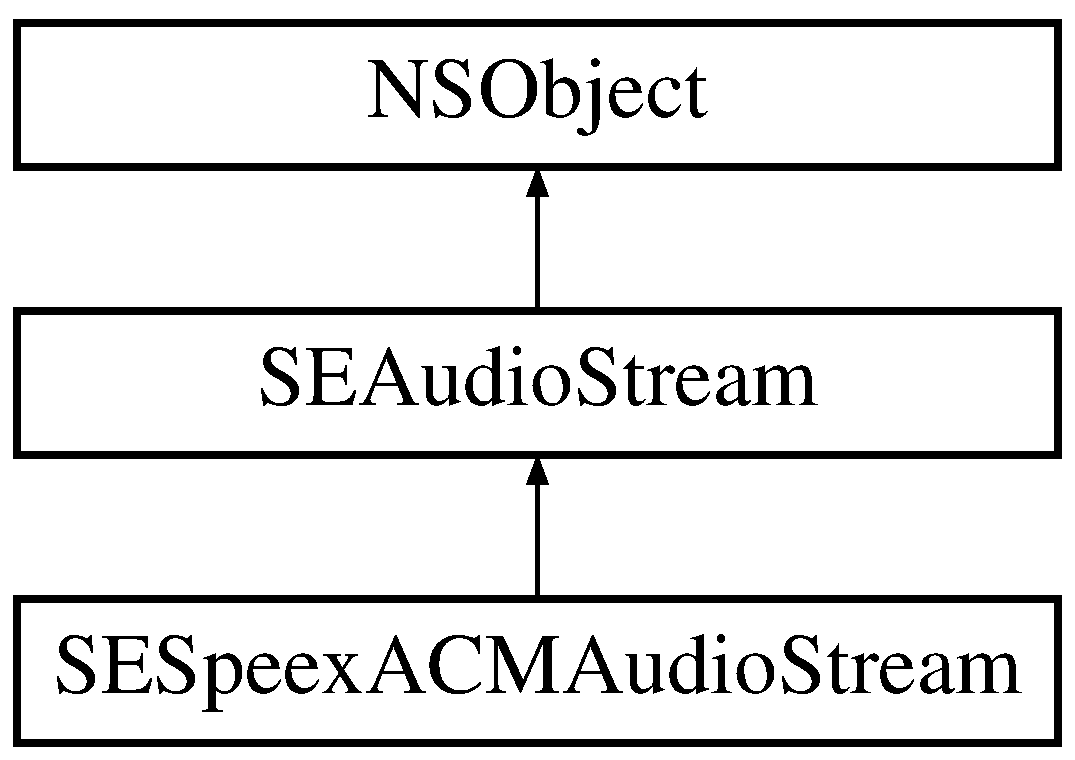
\includegraphics[height=3.000000cm]{interface_s_e_audio_stream}
\end{center}
\end{figure}
\subsection*{Instance Methods}
\begin{DoxyCompactItemize}
\item 
(id) -\/ \hyperlink{interface_s_e_audio_stream_adfb80527c355e64279d60a7b1af838ea}{init}
\item 
(id) -\/ \hyperlink{interface_s_e_audio_stream_a34663b1bbae1fdb5e32111a6629a994a}{init\-With\-Audio\-Stream\-:}
\item 
(id) -\/ \hyperlink{interface_s_e_audio_stream_a7acd0370d5f5066a6d00834af0eea200}{init\-With\-U\-R\-L\-:}
\item 
(id) -\/ \hyperlink{interface_s_e_audio_stream_a88b28dfe93892a08d261bd946beea26f}{init\-With\-Contents\-Of\-File\-:}
\item 
(void) -\/ \hyperlink{interface_s_e_audio_stream_add81dd9d9bd838f3a5dc1ceae94ccf26}{open}
\item 
(void) -\/ \hyperlink{interface_s_e_audio_stream_a8c4af367964e8be4817df12989f06d40}{close}
\item 
(void) -\/ \hyperlink{interface_s_e_audio_stream_ae59699f3f9cdf5fa000d9835da89e73e}{clear}
\item 
(void) -\/ \hyperlink{interface_s_e_audio_stream_a1dd26e76fbcd65f2d221f61de75fd3eb}{seek\-To\-Sample\-Position\-:}
\item 
(void) -\/ \hyperlink{interface_s_e_audio_stream_a720083efde7839f0a44ec7456805ffeb}{seek\-To\-Second\-:}
\item 
(void) -\/ \hyperlink{interface_s_e_audio_stream_ab721ccfe6c59695b85abc3fe00b37230}{exprort\-To\-File\-:completion\-:}
\item 
(N\-S\-Data $\ast$) -\/ \hyperlink{interface_s_e_audio_stream_a8d848d7a388d38fb670eb92e3bf6566d}{read\-Samples\-With\-Count\-:}
\item 
(N\-S\-Data $\ast$) -\/ \hyperlink{interface_s_e_audio_stream_a4501c22126f23cc1cb9ecbd1d7ddda6e}{read\-Samples\-From\-Channel\-:count\-:}
\item 
(void) -\/ \hyperlink{interface_s_e_audio_stream_ac80704c916ddbac8f8309f3a6a019e80}{read\-Samples\-:count\-:}
\item 
(void) -\/ \hyperlink{interface_s_e_audio_stream_ab184f74429643065a116a8f272bf79b3}{write\-Samples\-:}
\item 
(void) -\/ \hyperlink{interface_s_e_audio_stream_af19a129d2a78172d771f2552dd97f49b}{write\-Samples\-:count\-:}
\end{DoxyCompactItemize}
\subsection*{Properties}
\begin{DoxyCompactItemize}
\item 
Audio\-Stream\-Basic\-Description $\ast$ \hyperlink{interface_s_e_audio_stream_a96f11351b56bdd1d363ad05fb80d1a73}{audio\-Description}
\item 
N\-S\-Time\-Interval \hyperlink{interface_s_e_audio_stream_af5e4493693cf24fa25af34487993d693}{duration}
\item 
N\-S\-U\-R\-L $\ast$ \hyperlink{interface_s_e_audio_stream_a7561aaa75262c747a4da3d701e2094b9}{file\-Path\-U\-R\-L}
\item 
N\-S\-Error $\ast$ \hyperlink{interface_s_e_audio_stream_a095232a32323fc1b43568e1609cc934d}{error}
\item 
N\-S\-Integer \hyperlink{interface_s_e_audio_stream_a54229ab240455736790dad362c5335e1}{length}
\item 
N\-S\-Integer \hyperlink{interface_s_e_audio_stream_a1e8d0ba4849fffe376bcf5494987c9a8}{number\-Of\-Samples}
\item 
N\-S\-Integer \hyperlink{interface_s_e_audio_stream_afac964b9badc8642c250a2234eb3c044}{number\-Of\-Samples\-Per\-Channel}
\end{DoxyCompactItemize}


\subsection{Method Documentation}
\hypertarget{interface_s_e_audio_stream_ae59699f3f9cdf5fa000d9835da89e73e}{\index{S\-E\-Audio\-Stream@{S\-E\-Audio\-Stream}!clear@{clear}}
\index{clear@{clear}!SEAudioStream@{S\-E\-Audio\-Stream}}
\subsubsection[{clear}]{\setlength{\rightskip}{0pt plus 5cm}-\/ (void) clear 
\begin{DoxyParamCaption}
{}
\end{DoxyParamCaption}
}}\label{interface_s_e_audio_stream_ae59699f3f9cdf5fa000d9835da89e73e}
Delete all information in stream \hypertarget{interface_s_e_audio_stream_a8c4af367964e8be4817df12989f06d40}{\index{S\-E\-Audio\-Stream@{S\-E\-Audio\-Stream}!close@{close}}
\index{close@{close}!SEAudioStream@{S\-E\-Audio\-Stream}}
\subsubsection[{close}]{\setlength{\rightskip}{0pt plus 5cm}-\/ (void) close 
\begin{DoxyParamCaption}
{}
\end{DoxyParamCaption}
}}\label{interface_s_e_audio_stream_a8c4af367964e8be4817df12989f06d40}
Close Stream \hypertarget{interface_s_e_audio_stream_ab721ccfe6c59695b85abc3fe00b37230}{\index{S\-E\-Audio\-Stream@{S\-E\-Audio\-Stream}!exprort\-To\-File\-:completion\-:@{exprort\-To\-File\-:completion\-:}}
\index{exprort\-To\-File\-:completion\-:@{exprort\-To\-File\-:completion\-:}!SEAudioStream@{S\-E\-Audio\-Stream}}
\subsubsection[{exprort\-To\-File\-:completion\-:}]{\setlength{\rightskip}{0pt plus 5cm}-\/ (void) exprort\-To\-File\-: 
\begin{DoxyParamCaption}
\item[{(N\-S\-String$\ast$)}]{file\-Path}
\item[{completion:(void($^\wedge$)(N\-S\-Error$\ast$ {\bf error}))}]{completion}
\end{DoxyParamCaption}
}}\label{interface_s_e_audio_stream_ab721ccfe6c59695b85abc3fe00b37230}
Export all data to file \hypertarget{interface_s_e_audio_stream_adfb80527c355e64279d60a7b1af838ea}{\index{S\-E\-Audio\-Stream@{S\-E\-Audio\-Stream}!init@{init}}
\index{init@{init}!SEAudioStream@{S\-E\-Audio\-Stream}}
\subsubsection[{init}]{\setlength{\rightskip}{0pt plus 5cm}-\/ (id) init 
\begin{DoxyParamCaption}
{}
\end{DoxyParamCaption}
}}\label{interface_s_e_audio_stream_adfb80527c355e64279d60a7b1af838ea}
Create stream in memory \hypertarget{interface_s_e_audio_stream_a34663b1bbae1fdb5e32111a6629a994a}{\index{S\-E\-Audio\-Stream@{S\-E\-Audio\-Stream}!init\-With\-Audio\-Stream\-:@{init\-With\-Audio\-Stream\-:}}
\index{init\-With\-Audio\-Stream\-:@{init\-With\-Audio\-Stream\-:}!SEAudioStream@{S\-E\-Audio\-Stream}}
\subsubsection[{init\-With\-Audio\-Stream\-:}]{\setlength{\rightskip}{0pt plus 5cm}-\/ (id) init\-With\-Audio\-Stream\-: 
\begin{DoxyParamCaption}
\item[{({\bf S\-E\-Audio\-Stream}$\ast$)}]{stream}
\end{DoxyParamCaption}
}}\label{interface_s_e_audio_stream_a34663b1bbae1fdb5e32111a6629a994a}
Init with another audio stream \hypertarget{interface_s_e_audio_stream_a88b28dfe93892a08d261bd946beea26f}{\index{S\-E\-Audio\-Stream@{S\-E\-Audio\-Stream}!init\-With\-Contents\-Of\-File\-:@{init\-With\-Contents\-Of\-File\-:}}
\index{init\-With\-Contents\-Of\-File\-:@{init\-With\-Contents\-Of\-File\-:}!SEAudioStream@{S\-E\-Audio\-Stream}}
\subsubsection[{init\-With\-Contents\-Of\-File\-:}]{\setlength{\rightskip}{0pt plus 5cm}-\/ (id) init\-With\-Contents\-Of\-File\-: 
\begin{DoxyParamCaption}
\item[{(N\-S\-String$\ast$)}]{file}
\end{DoxyParamCaption}
}}\label{interface_s_e_audio_stream_a88b28dfe93892a08d261bd946beea26f}
Load from Storage \hypertarget{interface_s_e_audio_stream_a7acd0370d5f5066a6d00834af0eea200}{\index{S\-E\-Audio\-Stream@{S\-E\-Audio\-Stream}!init\-With\-U\-R\-L\-:@{init\-With\-U\-R\-L\-:}}
\index{init\-With\-U\-R\-L\-:@{init\-With\-U\-R\-L\-:}!SEAudioStream@{S\-E\-Audio\-Stream}}
\subsubsection[{init\-With\-U\-R\-L\-:}]{\setlength{\rightskip}{0pt plus 5cm}-\/ (id) init\-With\-U\-R\-L\-: 
\begin{DoxyParamCaption}
\item[{(N\-S\-String$\ast$)}]{url}
\end{DoxyParamCaption}
}}\label{interface_s_e_audio_stream_a7acd0370d5f5066a6d00834af0eea200}
Load from server \hypertarget{interface_s_e_audio_stream_add81dd9d9bd838f3a5dc1ceae94ccf26}{\index{S\-E\-Audio\-Stream@{S\-E\-Audio\-Stream}!open@{open}}
\index{open@{open}!SEAudioStream@{S\-E\-Audio\-Stream}}
\subsubsection[{open}]{\setlength{\rightskip}{0pt plus 5cm}-\/ (void) open 
\begin{DoxyParamCaption}
{}
\end{DoxyParamCaption}
}}\label{interface_s_e_audio_stream_add81dd9d9bd838f3a5dc1ceae94ccf26}
Open Stream \hypertarget{interface_s_e_audio_stream_ac80704c916ddbac8f8309f3a6a019e80}{\index{S\-E\-Audio\-Stream@{S\-E\-Audio\-Stream}!read\-Samples\-:count\-:@{read\-Samples\-:count\-:}}
\index{read\-Samples\-:count\-:@{read\-Samples\-:count\-:}!SEAudioStream@{S\-E\-Audio\-Stream}}
\subsubsection[{read\-Samples\-:count\-:}]{\setlength{\rightskip}{0pt plus 5cm}-\/ (void) read\-Samples\-: 
\begin{DoxyParamCaption}
\item[{(void $\ast$)}]{samples}
\item[{count:(N\-S\-Integer)}]{count}
\end{DoxyParamCaption}
}}\label{interface_s_e_audio_stream_ac80704c916ddbac8f8309f3a6a019e80}
Read Samples data 

Provided by category \hyperlink{category_s_e_audio_stream_07_read_08_ac80704c916ddbac8f8309f3a6a019e80}{S\-E\-Audio\-Stream(\-Read)}.

\hypertarget{interface_s_e_audio_stream_a4501c22126f23cc1cb9ecbd1d7ddda6e}{\index{S\-E\-Audio\-Stream@{S\-E\-Audio\-Stream}!read\-Samples\-From\-Channel\-:count\-:@{read\-Samples\-From\-Channel\-:count\-:}}
\index{read\-Samples\-From\-Channel\-:count\-:@{read\-Samples\-From\-Channel\-:count\-:}!SEAudioStream@{S\-E\-Audio\-Stream}}
\subsubsection[{read\-Samples\-From\-Channel\-:count\-:}]{\setlength{\rightskip}{0pt plus 5cm}-\/ (N\-S\-Data$\ast$) read\-Samples\-From\-Channel\-: 
\begin{DoxyParamCaption}
\item[{(N\-S\-Integer)}]{channels}
\item[{count:(N\-S\-Integer)}]{count}
\end{DoxyParamCaption}
}}\label{interface_s_e_audio_stream_a4501c22126f23cc1cb9ecbd1d7ddda6e}
Read Samples from one channel 

Provided by category \hyperlink{category_s_e_audio_stream_07_read_08_a4501c22126f23cc1cb9ecbd1d7ddda6e}{S\-E\-Audio\-Stream(\-Read)}.

\hypertarget{interface_s_e_audio_stream_a8d848d7a388d38fb670eb92e3bf6566d}{\index{S\-E\-Audio\-Stream@{S\-E\-Audio\-Stream}!read\-Samples\-With\-Count\-:@{read\-Samples\-With\-Count\-:}}
\index{read\-Samples\-With\-Count\-:@{read\-Samples\-With\-Count\-:}!SEAudioStream@{S\-E\-Audio\-Stream}}
\subsubsection[{read\-Samples\-With\-Count\-:}]{\setlength{\rightskip}{0pt plus 5cm}-\/ (N\-S\-Data$\ast$) read\-Samples\-With\-Count\-: 
\begin{DoxyParamCaption}
\item[{(N\-S\-Integer)}]{count}
\end{DoxyParamCaption}
}}\label{interface_s_e_audio_stream_a8d848d7a388d38fb670eb92e3bf6566d}
Read Samples from All Channels 

Provided by category \hyperlink{category_s_e_audio_stream_07_read_08_a8d848d7a388d38fb670eb92e3bf6566d}{S\-E\-Audio\-Stream(\-Read)}.

\hypertarget{interface_s_e_audio_stream_a1dd26e76fbcd65f2d221f61de75fd3eb}{\index{S\-E\-Audio\-Stream@{S\-E\-Audio\-Stream}!seek\-To\-Sample\-Position\-:@{seek\-To\-Sample\-Position\-:}}
\index{seek\-To\-Sample\-Position\-:@{seek\-To\-Sample\-Position\-:}!SEAudioStream@{S\-E\-Audio\-Stream}}
\subsubsection[{seek\-To\-Sample\-Position\-:}]{\setlength{\rightskip}{0pt plus 5cm}-\/ (void) seek\-To\-Sample\-Position\-: 
\begin{DoxyParamCaption}
\item[{(N\-S\-Integer)}]{position}
\end{DoxyParamCaption}
}}\label{interface_s_e_audio_stream_a1dd26e76fbcd65f2d221f61de75fd3eb}
Seek to position in samples include all channels \hypertarget{interface_s_e_audio_stream_a720083efde7839f0a44ec7456805ffeb}{\index{S\-E\-Audio\-Stream@{S\-E\-Audio\-Stream}!seek\-To\-Second\-:@{seek\-To\-Second\-:}}
\index{seek\-To\-Second\-:@{seek\-To\-Second\-:}!SEAudioStream@{S\-E\-Audio\-Stream}}
\subsubsection[{seek\-To\-Second\-:}]{\setlength{\rightskip}{0pt plus 5cm}-\/ (void) seek\-To\-Second\-: 
\begin{DoxyParamCaption}
\item[{(N\-S\-Time\-Interval)}]{second}
\end{DoxyParamCaption}
}}\label{interface_s_e_audio_stream_a720083efde7839f0a44ec7456805ffeb}
Seek to second \hypertarget{interface_s_e_audio_stream_ab184f74429643065a116a8f272bf79b3}{\index{S\-E\-Audio\-Stream@{S\-E\-Audio\-Stream}!write\-Samples\-:@{write\-Samples\-:}}
\index{write\-Samples\-:@{write\-Samples\-:}!SEAudioStream@{S\-E\-Audio\-Stream}}
\subsubsection[{write\-Samples\-:}]{\setlength{\rightskip}{0pt plus 5cm}-\/ (void) write\-Samples\-: 
\begin{DoxyParamCaption}
\item[{(N\-S\-Data $\ast$)}]{samples}
\end{DoxyParamCaption}
}}\label{interface_s_e_audio_stream_ab184f74429643065a116a8f272bf79b3}
Write Samples$\ast$ using N\-S\-Data 

Provided by category \hyperlink{category_s_e_audio_stream_07_write_08_ab184f74429643065a116a8f272bf79b3}{S\-E\-Audio\-Stream(\-Write)}.

\hypertarget{interface_s_e_audio_stream_af19a129d2a78172d771f2552dd97f49b}{\index{S\-E\-Audio\-Stream@{S\-E\-Audio\-Stream}!write\-Samples\-:count\-:@{write\-Samples\-:count\-:}}
\index{write\-Samples\-:count\-:@{write\-Samples\-:count\-:}!SEAudioStream@{S\-E\-Audio\-Stream}}
\subsubsection[{write\-Samples\-:count\-:}]{\setlength{\rightskip}{0pt plus 5cm}-\/ (void) {\bf write\-Samples\-:} 
\begin{DoxyParamCaption}
\item[{(void $\ast$)}]{data}
\item[{count:(N\-S\-Integer)}]{count}
\end{DoxyParamCaption}
}}\label{interface_s_e_audio_stream_af19a129d2a78172d771f2552dd97f49b}
Write Samples using data 

Provided by category \hyperlink{category_s_e_audio_stream_07_write_08_af19a129d2a78172d771f2552dd97f49b}{S\-E\-Audio\-Stream(\-Write)}.



\subsection{Property Documentation}
\hypertarget{interface_s_e_audio_stream_a96f11351b56bdd1d363ad05fb80d1a73}{\index{S\-E\-Audio\-Stream@{S\-E\-Audio\-Stream}!audio\-Description@{audio\-Description}}
\index{audio\-Description@{audio\-Description}!SEAudioStream@{S\-E\-Audio\-Stream}}
\subsubsection[{audio\-Description}]{\setlength{\rightskip}{0pt plus 5cm}-\/ (Audio\-Stream\-Basic\-Description$\ast$) audio\-Description\hspace{0.3cm}{\ttfamily [read]}, {\ttfamily [write]}, {\ttfamily [nonatomic]}, {\ttfamily [assign]}}}\label{interface_s_e_audio_stream_a96f11351b56bdd1d363ad05fb80d1a73}
Audio File Description \hypertarget{interface_s_e_audio_stream_af5e4493693cf24fa25af34487993d693}{\index{S\-E\-Audio\-Stream@{S\-E\-Audio\-Stream}!duration@{duration}}
\index{duration@{duration}!SEAudioStream@{S\-E\-Audio\-Stream}}
\subsubsection[{duration}]{\setlength{\rightskip}{0pt plus 5cm}-\/ (N\-S\-Time\-Interval) duration\hspace{0.3cm}{\ttfamily [read]}, {\ttfamily [nonatomic]}, {\ttfamily [assign]}}}\label{interface_s_e_audio_stream_af5e4493693cf24fa25af34487993d693}
Audio Duration$\ast$ \hypertarget{interface_s_e_audio_stream_a095232a32323fc1b43568e1609cc934d}{\index{S\-E\-Audio\-Stream@{S\-E\-Audio\-Stream}!error@{error}}
\index{error@{error}!SEAudioStream@{S\-E\-Audio\-Stream}}
\subsubsection[{error}]{\setlength{\rightskip}{0pt plus 5cm}-\/ (N\-S\-Error$\ast$) error\hspace{0.3cm}{\ttfamily [read]}, {\ttfamily [nonatomic]}, {\ttfamily [assign]}}}\label{interface_s_e_audio_stream_a095232a32323fc1b43568e1609cc934d}
Last Error \hypertarget{interface_s_e_audio_stream_a7561aaa75262c747a4da3d701e2094b9}{\index{S\-E\-Audio\-Stream@{S\-E\-Audio\-Stream}!file\-Path\-U\-R\-L@{file\-Path\-U\-R\-L}}
\index{file\-Path\-U\-R\-L@{file\-Path\-U\-R\-L}!SEAudioStream@{S\-E\-Audio\-Stream}}
\subsubsection[{file\-Path\-U\-R\-L}]{\setlength{\rightskip}{0pt plus 5cm}-\/ (N\-S\-U\-R\-L$\ast$) file\-Path\-U\-R\-L\hspace{0.3cm}{\ttfamily [read]}, {\ttfamily [nonatomic]}, {\ttfamily [assign]}}}\label{interface_s_e_audio_stream_a7561aaa75262c747a4da3d701e2094b9}
File Path \hypertarget{interface_s_e_audio_stream_a54229ab240455736790dad362c5335e1}{\index{S\-E\-Audio\-Stream@{S\-E\-Audio\-Stream}!length@{length}}
\index{length@{length}!SEAudioStream@{S\-E\-Audio\-Stream}}
\subsubsection[{length}]{\setlength{\rightskip}{0pt plus 5cm}-\/ (N\-S\-Integer) length\hspace{0.3cm}{\ttfamily [read]}, {\ttfamily [nonatomic]}, {\ttfamily [assign]}}}\label{interface_s_e_audio_stream_a54229ab240455736790dad362c5335e1}
Stream Length in bytes \hypertarget{interface_s_e_audio_stream_a1e8d0ba4849fffe376bcf5494987c9a8}{\index{S\-E\-Audio\-Stream@{S\-E\-Audio\-Stream}!number\-Of\-Samples@{number\-Of\-Samples}}
\index{number\-Of\-Samples@{number\-Of\-Samples}!SEAudioStream@{S\-E\-Audio\-Stream}}
\subsubsection[{number\-Of\-Samples}]{\setlength{\rightskip}{0pt plus 5cm}-\/ (N\-S\-Integer) number\-Of\-Samples\hspace{0.3cm}{\ttfamily [read]}, {\ttfamily [nonatomic]}, {\ttfamily [assign]}}}\label{interface_s_e_audio_stream_a1e8d0ba4849fffe376bcf5494987c9a8}
Number of samples including all channels \hypertarget{interface_s_e_audio_stream_afac964b9badc8642c250a2234eb3c044}{\index{S\-E\-Audio\-Stream@{S\-E\-Audio\-Stream}!number\-Of\-Samples\-Per\-Channel@{number\-Of\-Samples\-Per\-Channel}}
\index{number\-Of\-Samples\-Per\-Channel@{number\-Of\-Samples\-Per\-Channel}!SEAudioStream@{S\-E\-Audio\-Stream}}
\subsubsection[{number\-Of\-Samples\-Per\-Channel}]{\setlength{\rightskip}{0pt plus 5cm}-\/ (N\-S\-Integer) number\-Of\-Samples\-Per\-Channel\hspace{0.3cm}{\ttfamily [read]}, {\ttfamily [nonatomic]}, {\ttfamily [assign]}}}\label{interface_s_e_audio_stream_afac964b9badc8642c250a2234eb3c044}
Number of samples per channel 

The documentation for this class was generated from the following files\-:\begin{DoxyCompactItemize}
\item 
/\-Users/igor/\-Develop/\-Develop\-Git/\-Davacon/i\-Phone/\-Sound\-Recorder/\-Classes/\-Core/\-Sound\-Editor/\hyperlink{_s_e_audio_stream_8h}{S\-E\-Audio\-Stream.\-h}\item 
/\-Users/igor/\-Develop/\-Develop\-Git/\-Davacon/i\-Phone/\-Sound\-Recorder/\-Classes/\-Core/\-Sound\-Editor/\hyperlink{_s_e_audio_stream_8m}{S\-E\-Audio\-Stream.\-m}\end{DoxyCompactItemize}

\hypertarget{category_s_e_audio_stream_07_read_08}{\section{S\-E\-Audio\-Stream(Read) Category Reference}
\label{category_s_e_audio_stream_07_read_08}\index{S\-E\-Audio\-Stream(\-Read)@{S\-E\-Audio\-Stream(\-Read)}}
}


{\ttfamily \#import $<$S\-E\-Audio\-Stream.\-h$>$}

\subsection*{Instance Methods}
\begin{DoxyCompactItemize}
\item 
(N\-S\-Data $\ast$) -\/ \hyperlink{category_s_e_audio_stream_07_read_08_a8d848d7a388d38fb670eb92e3bf6566d}{read\-Samples\-With\-Count\-:}
\item 
(N\-S\-Data $\ast$) -\/ \hyperlink{category_s_e_audio_stream_07_read_08_a4501c22126f23cc1cb9ecbd1d7ddda6e}{read\-Samples\-From\-Channel\-:count\-:}
\item 
(void) -\/ \hyperlink{category_s_e_audio_stream_07_read_08_ac80704c916ddbac8f8309f3a6a019e80}{read\-Samples\-:count\-:}
\end{DoxyCompactItemize}


\subsection{Method Documentation}
\hypertarget{category_s_e_audio_stream_07_read_08_ac80704c916ddbac8f8309f3a6a019e80}{\index{S\-E\-Audio\-Stream(\-Read)@{S\-E\-Audio\-Stream(\-Read)}!read\-Samples\-:count\-:@{read\-Samples\-:count\-:}}
\index{read\-Samples\-:count\-:@{read\-Samples\-:count\-:}!SEAudioStream(Read)@{S\-E\-Audio\-Stream(\-Read)}}
\subsubsection[{read\-Samples\-:count\-:}]{\setlength{\rightskip}{0pt plus 5cm}-\/ (void) read\-Samples\-: 
\begin{DoxyParamCaption}
\item[{(void $\ast$)}]{samples}
\item[{count:(N\-S\-Integer)}]{count}
\end{DoxyParamCaption}
}}\label{category_s_e_audio_stream_07_read_08_ac80704c916ddbac8f8309f3a6a019e80}
Read Samples data 

Extends class \hyperlink{interface_s_e_audio_stream_ac80704c916ddbac8f8309f3a6a019e80}{S\-E\-Audio\-Stream}.

\hypertarget{category_s_e_audio_stream_07_read_08_a4501c22126f23cc1cb9ecbd1d7ddda6e}{\index{S\-E\-Audio\-Stream(\-Read)@{S\-E\-Audio\-Stream(\-Read)}!read\-Samples\-From\-Channel\-:count\-:@{read\-Samples\-From\-Channel\-:count\-:}}
\index{read\-Samples\-From\-Channel\-:count\-:@{read\-Samples\-From\-Channel\-:count\-:}!SEAudioStream(Read)@{S\-E\-Audio\-Stream(\-Read)}}
\subsubsection[{read\-Samples\-From\-Channel\-:count\-:}]{\setlength{\rightskip}{0pt plus 5cm}-\/ (N\-S\-Data$\ast$) read\-Samples\-From\-Channel\-: 
\begin{DoxyParamCaption}
\item[{(N\-S\-Integer)}]{channels}
\item[{count:(N\-S\-Integer)}]{count}
\end{DoxyParamCaption}
}}\label{category_s_e_audio_stream_07_read_08_a4501c22126f23cc1cb9ecbd1d7ddda6e}
Read Samples from one channel 

Extends class \hyperlink{interface_s_e_audio_stream_a4501c22126f23cc1cb9ecbd1d7ddda6e}{S\-E\-Audio\-Stream}.

\hypertarget{category_s_e_audio_stream_07_read_08_a8d848d7a388d38fb670eb92e3bf6566d}{\index{S\-E\-Audio\-Stream(\-Read)@{S\-E\-Audio\-Stream(\-Read)}!read\-Samples\-With\-Count\-:@{read\-Samples\-With\-Count\-:}}
\index{read\-Samples\-With\-Count\-:@{read\-Samples\-With\-Count\-:}!SEAudioStream(Read)@{S\-E\-Audio\-Stream(\-Read)}}
\subsubsection[{read\-Samples\-With\-Count\-:}]{\setlength{\rightskip}{0pt plus 5cm}-\/ (N\-S\-Data$\ast$) read\-Samples\-With\-Count\-: 
\begin{DoxyParamCaption}
\item[{(N\-S\-Integer)}]{count}
\end{DoxyParamCaption}
}}\label{category_s_e_audio_stream_07_read_08_a8d848d7a388d38fb670eb92e3bf6566d}
Read Samples from All Channels 

Extends class \hyperlink{interface_s_e_audio_stream_a8d848d7a388d38fb670eb92e3bf6566d}{S\-E\-Audio\-Stream}.



The documentation for this category was generated from the following file\-:\begin{DoxyCompactItemize}
\item 
/\-Users/igor/\-Develop/\-Develop\-Git/\-Davacon/i\-Phone/\-Sound\-Recorder/\-Classes/\-Core/\-Sound\-Editor/\hyperlink{_s_e_audio_stream_8h}{S\-E\-Audio\-Stream.\-h}\end{DoxyCompactItemize}

\hypertarget{category_s_e_audio_stream_07_write_08}{\section{S\-E\-Audio\-Stream(Write) Category Reference}
\label{category_s_e_audio_stream_07_write_08}\index{S\-E\-Audio\-Stream(\-Write)@{S\-E\-Audio\-Stream(\-Write)}}
}


{\ttfamily \#import $<$S\-E\-Audio\-Stream.\-h$>$}

\subsection*{Instance Methods}
\begin{DoxyCompactItemize}
\item 
(void) -\/ \hyperlink{category_s_e_audio_stream_07_write_08_ab184f74429643065a116a8f272bf79b3}{write\-Samples\-:}
\item 
(void) -\/ \hyperlink{category_s_e_audio_stream_07_write_08_af19a129d2a78172d771f2552dd97f49b}{write\-Samples\-:count\-:}
\end{DoxyCompactItemize}


\subsection{Method Documentation}
\hypertarget{category_s_e_audio_stream_07_write_08_ab184f74429643065a116a8f272bf79b3}{\index{S\-E\-Audio\-Stream(\-Write)@{S\-E\-Audio\-Stream(\-Write)}!write\-Samples\-:@{write\-Samples\-:}}
\index{write\-Samples\-:@{write\-Samples\-:}!SEAudioStream(Write)@{S\-E\-Audio\-Stream(\-Write)}}
\subsubsection[{write\-Samples\-:}]{\setlength{\rightskip}{0pt plus 5cm}-\/ (void) write\-Samples\-: 
\begin{DoxyParamCaption}
\item[{(N\-S\-Data $\ast$)}]{samples}
\end{DoxyParamCaption}
}}\label{category_s_e_audio_stream_07_write_08_ab184f74429643065a116a8f272bf79b3}
Write Samples$\ast$ using N\-S\-Data 

Extends class \hyperlink{interface_s_e_audio_stream_ab184f74429643065a116a8f272bf79b3}{S\-E\-Audio\-Stream}.

\hypertarget{category_s_e_audio_stream_07_write_08_af19a129d2a78172d771f2552dd97f49b}{\index{S\-E\-Audio\-Stream(\-Write)@{S\-E\-Audio\-Stream(\-Write)}!write\-Samples\-:count\-:@{write\-Samples\-:count\-:}}
\index{write\-Samples\-:count\-:@{write\-Samples\-:count\-:}!SEAudioStream(Write)@{S\-E\-Audio\-Stream(\-Write)}}
\subsubsection[{write\-Samples\-:count\-:}]{\setlength{\rightskip}{0pt plus 5cm}-\/ (void) write\-Samples\-: 
\begin{DoxyParamCaption}
\item[{(void $\ast$)}]{data}
\item[{count:(N\-S\-Integer)}]{count}
\end{DoxyParamCaption}
}}\label{category_s_e_audio_stream_07_write_08_af19a129d2a78172d771f2552dd97f49b}
Write Samples using data 

Extends class \hyperlink{interface_s_e_audio_stream_af19a129d2a78172d771f2552dd97f49b}{S\-E\-Audio\-Stream}.



The documentation for this category was generated from the following file\-:\begin{DoxyCompactItemize}
\item 
/\-Users/igor/\-Develop/\-Develop\-Git/\-Davacon/i\-Phone/\-Sound\-Recorder/\-Classes/\-Core/\-Sound\-Editor/\hyperlink{_s_e_audio_stream_8h}{S\-E\-Audio\-Stream.\-h}\end{DoxyCompactItemize}

\hypertarget{interface_s_e_audio_stream_player}{\section{S\-E\-Audio\-Stream\-Player Class Reference}
\label{interface_s_e_audio_stream_player}\index{S\-E\-Audio\-Stream\-Player@{S\-E\-Audio\-Stream\-Player}}
}


{\ttfamily \#import $<$S\-E\-Audio\-Stream\-Player.\-h$>$}

Inheritance diagram for S\-E\-Audio\-Stream\-Player\-:\begin{figure}[H]
\begin{center}
\leavevmode
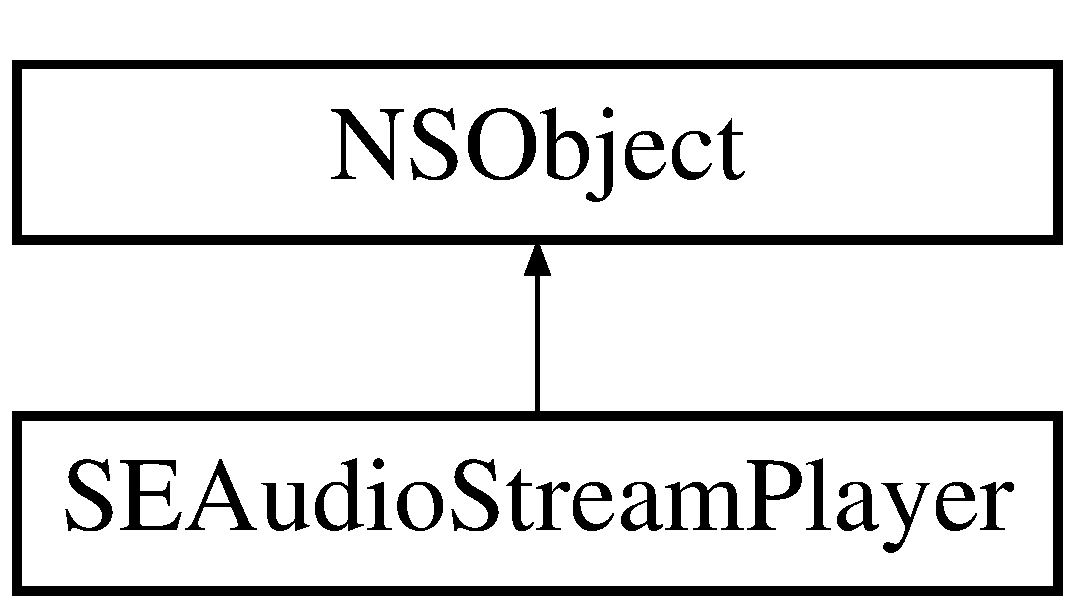
\includegraphics[height=2.000000cm]{interface_s_e_audio_stream_player}
\end{center}
\end{figure}
\subsection*{Instance Methods}
\begin{DoxyCompactItemize}
\item 
(id) -\/ \hyperlink{interface_s_e_audio_stream_player_af81895d0a82b3255e9b9840def52599b}{init\-With\-Stream\-:}
\item 
(void) -\/ \hyperlink{interface_s_e_audio_stream_player_a16c600129d3045dc7f7213165df3ca66}{start}
\item 
(void) -\/ \hyperlink{interface_s_e_audio_stream_player_ab9e4c08bf6710368576d15ea05ecfe32}{pause}
\item 
(void) -\/ \hyperlink{interface_s_e_audio_stream_player_a80491754758a4dab432e18fcafb0721d}{stop}
\end{DoxyCompactItemize}
\subsection*{Properties}
\begin{DoxyCompactItemize}
\item 
id$<$ \hyperlink{protocol_s_e_audio_stream_player_delegate-p}{S\-E\-Audio\-Stream\-Player\-Delegate} $>$ \hyperlink{interface_s_e_audio_stream_player_a423b5909f11bd592bbef74ac92b18a30}{delegate}
\item 
B\-O\-O\-L \hyperlink{interface_s_e_audio_stream_player_ae9c780174af7f5d4bbd970049f7d1bb5}{is\-Playing}
\item 
B\-O\-O\-L \hyperlink{interface_s_e_audio_stream_player_ad6bec3654ff73d3fd4d11111a1f69442}{is\-Paused}
\item 
N\-S\-Time\-Interval \hyperlink{interface_s_e_audio_stream_player_a079874e98c33b3fc543f9ca6ea2a59e7}{current\-Time}
\end{DoxyCompactItemize}


\subsection{Method Documentation}
\hypertarget{interface_s_e_audio_stream_player_af81895d0a82b3255e9b9840def52599b}{\index{S\-E\-Audio\-Stream\-Player@{S\-E\-Audio\-Stream\-Player}!init\-With\-Stream\-:@{init\-With\-Stream\-:}}
\index{init\-With\-Stream\-:@{init\-With\-Stream\-:}!SEAudioStreamPlayer@{S\-E\-Audio\-Stream\-Player}}
\subsubsection[{init\-With\-Stream\-:}]{\setlength{\rightskip}{0pt plus 5cm}-\/ (id) init\-With\-Stream\-: 
\begin{DoxyParamCaption}
\item[{({\bf S\-E\-Audio\-Stream} $\ast$)}]{stream}
\end{DoxyParamCaption}
}}\label{interface_s_e_audio_stream_player_af81895d0a82b3255e9b9840def52599b}
\hypertarget{interface_s_e_audio_stream_player_ab9e4c08bf6710368576d15ea05ecfe32}{\index{S\-E\-Audio\-Stream\-Player@{S\-E\-Audio\-Stream\-Player}!pause@{pause}}
\index{pause@{pause}!SEAudioStreamPlayer@{S\-E\-Audio\-Stream\-Player}}
\subsubsection[{pause}]{\setlength{\rightskip}{0pt plus 5cm}-\/ (void) pause 
\begin{DoxyParamCaption}
{}
\end{DoxyParamCaption}
}}\label{interface_s_e_audio_stream_player_ab9e4c08bf6710368576d15ea05ecfe32}
\hypertarget{interface_s_e_audio_stream_player_a16c600129d3045dc7f7213165df3ca66}{\index{S\-E\-Audio\-Stream\-Player@{S\-E\-Audio\-Stream\-Player}!start@{start}}
\index{start@{start}!SEAudioStreamPlayer@{S\-E\-Audio\-Stream\-Player}}
\subsubsection[{start}]{\setlength{\rightskip}{0pt plus 5cm}-\/ (void) start 
\begin{DoxyParamCaption}
{}
\end{DoxyParamCaption}
}}\label{interface_s_e_audio_stream_player_a16c600129d3045dc7f7213165df3ca66}
\hypertarget{interface_s_e_audio_stream_player_a80491754758a4dab432e18fcafb0721d}{\index{S\-E\-Audio\-Stream\-Player@{S\-E\-Audio\-Stream\-Player}!stop@{stop}}
\index{stop@{stop}!SEAudioStreamPlayer@{S\-E\-Audio\-Stream\-Player}}
\subsubsection[{stop}]{\setlength{\rightskip}{0pt plus 5cm}-\/ (void) stop 
\begin{DoxyParamCaption}
{}
\end{DoxyParamCaption}
}}\label{interface_s_e_audio_stream_player_a80491754758a4dab432e18fcafb0721d}


\subsection{Property Documentation}
\hypertarget{interface_s_e_audio_stream_player_a079874e98c33b3fc543f9ca6ea2a59e7}{\index{S\-E\-Audio\-Stream\-Player@{S\-E\-Audio\-Stream\-Player}!current\-Time@{current\-Time}}
\index{current\-Time@{current\-Time}!SEAudioStreamPlayer@{S\-E\-Audio\-Stream\-Player}}
\subsubsection[{current\-Time}]{\setlength{\rightskip}{0pt plus 5cm}-\/ (N\-S\-Time\-Interval) current\-Time\hspace{0.3cm}{\ttfamily [read]}, {\ttfamily [write]}, {\ttfamily [nonatomic]}, {\ttfamily [assign]}}}\label{interface_s_e_audio_stream_player_a079874e98c33b3fc543f9ca6ea2a59e7}
\hypertarget{interface_s_e_audio_stream_player_a423b5909f11bd592bbef74ac92b18a30}{\index{S\-E\-Audio\-Stream\-Player@{S\-E\-Audio\-Stream\-Player}!delegate@{delegate}}
\index{delegate@{delegate}!SEAudioStreamPlayer@{S\-E\-Audio\-Stream\-Player}}
\subsubsection[{delegate}]{\setlength{\rightskip}{0pt plus 5cm}-\/ (id$<${\bf S\-E\-Audio\-Stream\-Player\-Delegate}$>$) delegate\hspace{0.3cm}{\ttfamily [read]}, {\ttfamily [write]}, {\ttfamily [nonatomic]}, {\ttfamily [weak]}}}\label{interface_s_e_audio_stream_player_a423b5909f11bd592bbef74ac92b18a30}
\hypertarget{interface_s_e_audio_stream_player_ad6bec3654ff73d3fd4d11111a1f69442}{\index{S\-E\-Audio\-Stream\-Player@{S\-E\-Audio\-Stream\-Player}!is\-Paused@{is\-Paused}}
\index{is\-Paused@{is\-Paused}!SEAudioStreamPlayer@{S\-E\-Audio\-Stream\-Player}}
\subsubsection[{is\-Paused}]{\setlength{\rightskip}{0pt plus 5cm}-\/ (B\-O\-O\-L) is\-Paused\hspace{0.3cm}{\ttfamily [read]}, {\ttfamily [nonatomic]}, {\ttfamily [assign]}}}\label{interface_s_e_audio_stream_player_ad6bec3654ff73d3fd4d11111a1f69442}
\hypertarget{interface_s_e_audio_stream_player_ae9c780174af7f5d4bbd970049f7d1bb5}{\index{S\-E\-Audio\-Stream\-Player@{S\-E\-Audio\-Stream\-Player}!is\-Playing@{is\-Playing}}
\index{is\-Playing@{is\-Playing}!SEAudioStreamPlayer@{S\-E\-Audio\-Stream\-Player}}
\subsubsection[{is\-Playing}]{\setlength{\rightskip}{0pt plus 5cm}-\/ (B\-O\-O\-L) is\-Playing\hspace{0.3cm}{\ttfamily [read]}, {\ttfamily [nonatomic]}, {\ttfamily [assign]}}}\label{interface_s_e_audio_stream_player_ae9c780174af7f5d4bbd970049f7d1bb5}


The documentation for this class was generated from the following file\-:\begin{DoxyCompactItemize}
\item 
Sound\-Recorder/\-Classes/\-Core/\-Sound\-Editor/\hyperlink{_s_e_audio_stream_player_8h}{S\-E\-Audio\-Stream\-Player.\-h}\end{DoxyCompactItemize}

\hypertarget{protocol_s_e_audio_stream_player_delegate-p}{\section{$<$S\-E\-Audio\-Stream\-Player\-Delegate$>$ Protocol Reference}
\label{protocol_s_e_audio_stream_player_delegate-p}\index{$<$\-S\-E\-Audio\-Stream\-Player\-Delegate$>$@{$<$\-S\-E\-Audio\-Stream\-Player\-Delegate$>$}}
}


{\ttfamily \#import $<$S\-E\-Audio\-Stream\-Player.\-h$>$}



Inheritance diagram for $<$S\-E\-Audio\-Stream\-Player\-Delegate$>$\-:


Collaboration diagram for $<$S\-E\-Audio\-Stream\-Player\-Delegate$>$\-:
\subsection*{Instance Methods}
\begin{DoxyCompactItemize}
\item 
(void) -\/ \hyperlink{protocol_s_e_audio_stream_player_delegate-p_a74bb3b4dcd45b0c79616eba1d11fdd02}{audio\-Stream\-Player\-Did\-Start\-Playing\-:}
\item 
(void) -\/ \hyperlink{protocol_s_e_audio_stream_player_delegate-p_a11ec4e64acd6d9a5bc84a94a314c4335}{audio\-Stream\-Player\-Did\-Pause\-:}
\item 
(void) -\/ \hyperlink{protocol_s_e_audio_stream_player_delegate-p_abbf414d9214d2bae34556952792fa8bc}{audio\-Stream\-Player\-Did\-Continue\-:}
\item 
(void) -\/ \hyperlink{protocol_s_e_audio_stream_player_delegate-p_a16a6ec647062ed75001f394ae08a1125}{audio\-Stream\-Player\-:did\-Update\-With\-Current\-Position\-:duration\-:}
\item 
(void) -\/ \hyperlink{protocol_s_e_audio_stream_player_delegate-p_afd0e13575d327b091285b6c7f44792d3}{audio\-Stream\-Player\-Did\-Finish\-Playing\-:stopped\-:}
\end{DoxyCompactItemize}


\subsection{Method Documentation}
\hypertarget{protocol_s_e_audio_stream_player_delegate-p_a16a6ec647062ed75001f394ae08a1125}{\index{S\-E\-Audio\-Stream\-Player\-Delegate-\/p@{S\-E\-Audio\-Stream\-Player\-Delegate-\/p}!audio\-Stream\-Player\-:did\-Update\-With\-Current\-Position\-:duration\-:@{audio\-Stream\-Player\-:did\-Update\-With\-Current\-Position\-:duration\-:}}
\index{audio\-Stream\-Player\-:did\-Update\-With\-Current\-Position\-:duration\-:@{audio\-Stream\-Player\-:did\-Update\-With\-Current\-Position\-:duration\-:}!SEAudioStreamPlayerDelegate-p@{S\-E\-Audio\-Stream\-Player\-Delegate-\/p}}
\subsubsection[{audio\-Stream\-Player\-:did\-Update\-With\-Current\-Position\-:duration\-:}]{\setlength{\rightskip}{0pt plus 5cm}-\/ (void) audio\-Stream\-Player\-: 
\begin{DoxyParamCaption}
\item[{({\bf S\-E\-Audio\-Stream\-Player} $\ast$)}]{player}
\item[{didUpdateWithCurrentPosition:(N\-S\-Time\-Interval)}]{positon}
\item[{duration:(N\-S\-Time\-Interval)}]{duration}
\end{DoxyParamCaption}
}}\label{protocol_s_e_audio_stream_player_delegate-p_a16a6ec647062ed75001f394ae08a1125}
Notification for updating info about play state \hypertarget{protocol_s_e_audio_stream_player_delegate-p_abbf414d9214d2bae34556952792fa8bc}{\index{S\-E\-Audio\-Stream\-Player\-Delegate-\/p@{S\-E\-Audio\-Stream\-Player\-Delegate-\/p}!audio\-Stream\-Player\-Did\-Continue\-:@{audio\-Stream\-Player\-Did\-Continue\-:}}
\index{audio\-Stream\-Player\-Did\-Continue\-:@{audio\-Stream\-Player\-Did\-Continue\-:}!SEAudioStreamPlayerDelegate-p@{S\-E\-Audio\-Stream\-Player\-Delegate-\/p}}
\subsubsection[{audio\-Stream\-Player\-Did\-Continue\-:}]{\setlength{\rightskip}{0pt plus 5cm}-\/ (void) audio\-Stream\-Player\-Did\-Continue\-: 
\begin{DoxyParamCaption}
\item[{({\bf S\-E\-Audio\-Stream\-Player} $\ast$)}]{player}
\end{DoxyParamCaption}
}}\label{protocol_s_e_audio_stream_player_delegate-p_abbf414d9214d2bae34556952792fa8bc}
Notification for continue playing after pause \hypertarget{protocol_s_e_audio_stream_player_delegate-p_afd0e13575d327b091285b6c7f44792d3}{\index{S\-E\-Audio\-Stream\-Player\-Delegate-\/p@{S\-E\-Audio\-Stream\-Player\-Delegate-\/p}!audio\-Stream\-Player\-Did\-Finish\-Playing\-:stopped\-:@{audio\-Stream\-Player\-Did\-Finish\-Playing\-:stopped\-:}}
\index{audio\-Stream\-Player\-Did\-Finish\-Playing\-:stopped\-:@{audio\-Stream\-Player\-Did\-Finish\-Playing\-:stopped\-:}!SEAudioStreamPlayerDelegate-p@{S\-E\-Audio\-Stream\-Player\-Delegate-\/p}}
\subsubsection[{audio\-Stream\-Player\-Did\-Finish\-Playing\-:stopped\-:}]{\setlength{\rightskip}{0pt plus 5cm}-\/ (void) audio\-Stream\-Player\-Did\-Finish\-Playing\-: 
\begin{DoxyParamCaption}
\item[{({\bf S\-E\-Audio\-Stream\-Player} $\ast$)}]{player}
\item[{stopped:(B\-O\-O\-L)}]{stopped}
\end{DoxyParamCaption}
}}\label{protocol_s_e_audio_stream_player_delegate-p_afd0e13575d327b091285b6c7f44792d3}
Notification for end playing \hypertarget{protocol_s_e_audio_stream_player_delegate-p_a11ec4e64acd6d9a5bc84a94a314c4335}{\index{S\-E\-Audio\-Stream\-Player\-Delegate-\/p@{S\-E\-Audio\-Stream\-Player\-Delegate-\/p}!audio\-Stream\-Player\-Did\-Pause\-:@{audio\-Stream\-Player\-Did\-Pause\-:}}
\index{audio\-Stream\-Player\-Did\-Pause\-:@{audio\-Stream\-Player\-Did\-Pause\-:}!SEAudioStreamPlayerDelegate-p@{S\-E\-Audio\-Stream\-Player\-Delegate-\/p}}
\subsubsection[{audio\-Stream\-Player\-Did\-Pause\-:}]{\setlength{\rightskip}{0pt plus 5cm}-\/ (void) audio\-Stream\-Player\-Did\-Pause\-: 
\begin{DoxyParamCaption}
\item[{({\bf S\-E\-Audio\-Stream\-Player} $\ast$)}]{player}
\end{DoxyParamCaption}
}}\label{protocol_s_e_audio_stream_player_delegate-p_a11ec4e64acd6d9a5bc84a94a314c4335}
Notification for pause playing \hypertarget{protocol_s_e_audio_stream_player_delegate-p_a74bb3b4dcd45b0c79616eba1d11fdd02}{\index{S\-E\-Audio\-Stream\-Player\-Delegate-\/p@{S\-E\-Audio\-Stream\-Player\-Delegate-\/p}!audio\-Stream\-Player\-Did\-Start\-Playing\-:@{audio\-Stream\-Player\-Did\-Start\-Playing\-:}}
\index{audio\-Stream\-Player\-Did\-Start\-Playing\-:@{audio\-Stream\-Player\-Did\-Start\-Playing\-:}!SEAudioStreamPlayerDelegate-p@{S\-E\-Audio\-Stream\-Player\-Delegate-\/p}}
\subsubsection[{audio\-Stream\-Player\-Did\-Start\-Playing\-:}]{\setlength{\rightskip}{0pt plus 5cm}-\/ (void) audio\-Stream\-Player\-Did\-Start\-Playing\-: 
\begin{DoxyParamCaption}
\item[{({\bf S\-E\-Audio\-Stream\-Player} $\ast$)}]{player}
\end{DoxyParamCaption}
}}\label{protocol_s_e_audio_stream_player_delegate-p_a74bb3b4dcd45b0c79616eba1d11fdd02}
Notification for begin playing 

The documentation for this protocol was generated from the following file\-:\begin{DoxyCompactItemize}
\item 
/\-Users/igor/\-Develop/\-Develop\-Git/\-Davacon/i\-Phone/\-Sound\-Recorder/\-Classes/\-Core/\-Sound\-Editor/\hyperlink{_s_e_audio_stream_player_8h}{S\-E\-Audio\-Stream\-Player.\-h}\end{DoxyCompactItemize}

\hypertarget{interface_s_e_project}{\section{S\-E\-Project Class Reference}
\label{interface_s_e_project}\index{S\-E\-Project@{S\-E\-Project}}
}


{\ttfamily \#import $<$S\-E\-Project.\-h$>$}

Inheritance diagram for S\-E\-Project\-:\begin{figure}[H]
\begin{center}
\leavevmode
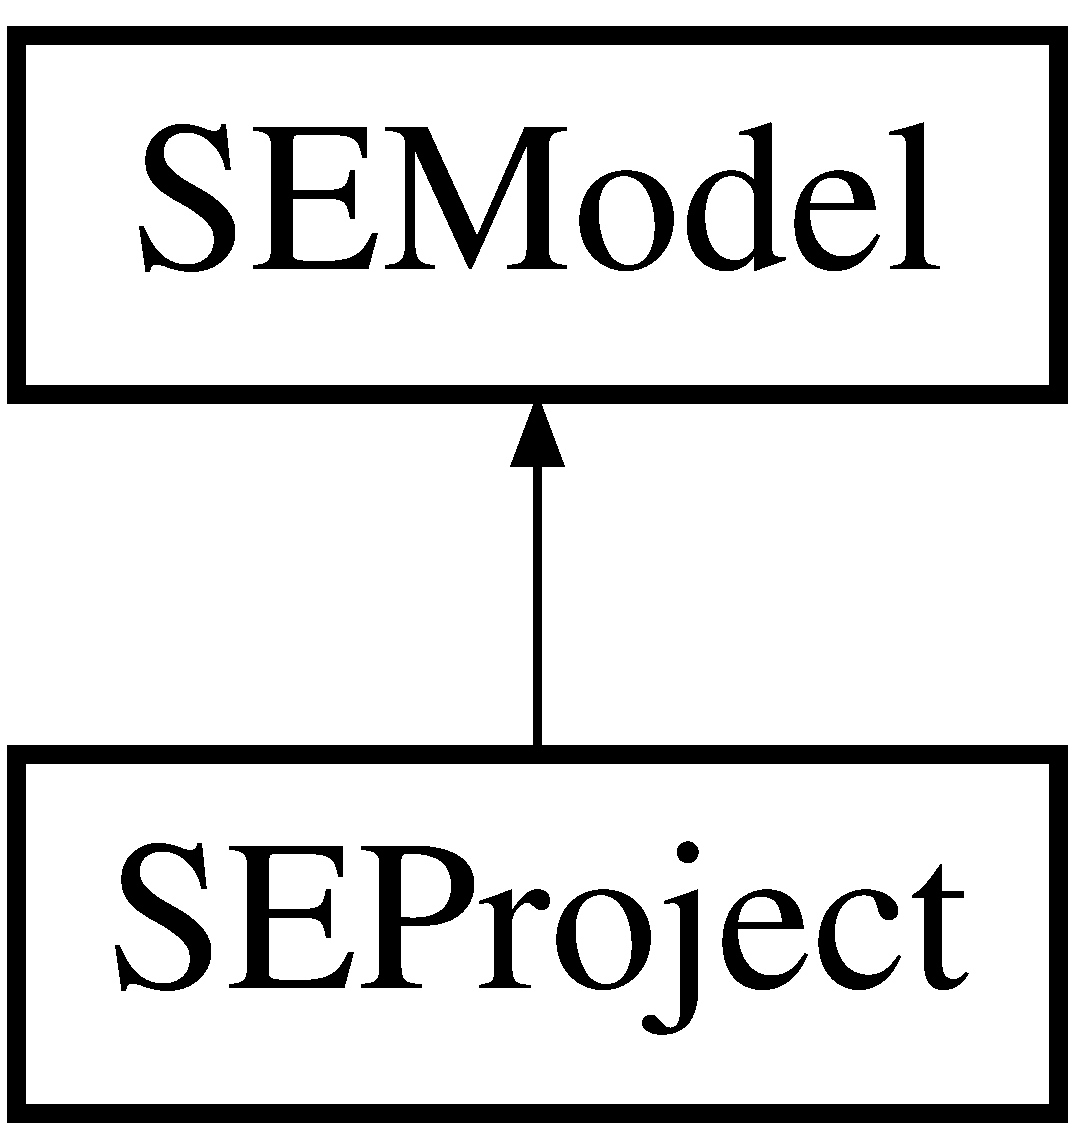
\includegraphics[height=2.000000cm]{interface_s_e_project}
\end{center}
\end{figure}
\subsection*{Instance Methods}
\begin{DoxyCompactItemize}
\item 
(\hyperlink{interface_s_e_record}{S\-E\-Record} $\ast$) -\/ \hyperlink{interface_s_e_project_adb4519610c7481bf048f235189ff737c}{split\-Record\-In\-Position\-:}
\item 
(void) -\/ \hyperlink{interface_s_e_project_a215f3b65a6214364b1c91a3e868e326f}{add\-Record\-:}
\item 
(void) -\/ \hyperlink{interface_s_e_project_a766d033976c34b25c714664a936431c0}{delete\-Record\-:}
\item 
(void) -\/ \hyperlink{interface_s_e_project_a6df677b3addadd2b57c7cb476817b3f0}{move\-Record\-:to\-Index\-:}
\item 
(void) -\/ \hyperlink{interface_s_e_project_adf1f53d931f669b12dfbabf92e3e90a4}{remove\-All\-Records}
\item 
(void) -\/ \hyperlink{interface_s_e_project_ad0dc83a89c70e8a670d2e0eb0381e632}{save\-Project}
\item 
(void) -\/ \hyperlink{interface_s_e_project_a996a39778f2d176ecf7ffda117703f6c}{save\-Project\-Asynchronously\-With\-Completion\-:}
\end{DoxyCompactItemize}
\subsection*{Properties}
\begin{DoxyCompactItemize}
\item 
N\-S\-String $\ast$ \hyperlink{interface_s_e_project_adf05552fc2cf324eb3511d3bd1b8a996}{name}
\item 
N\-S\-String $\ast$ \hyperlink{interface_s_e_project_a2d54ed4720974d226ab30b8d32ef21dd}{project\-File\-Path}
\item 
N\-S\-String $\ast$ \hyperlink{interface_s_e_project_a59726fcb927ff059c83a1ac7b252db0d}{project\-Sounds\-Path}
\item 
N\-S\-Array $\ast$ \hyperlink{interface_s_e_project_ac1f0c37f5832b2ba24ac9bf65f0fdcce}{records}
\item 
\hyperlink{interface_s_e_audio_stream_player}{S\-E\-Audio\-Stream\-Player} $\ast$ \hyperlink{interface_s_e_project_af35059bb818d498c8a96053818016a26}{audio\-Stream}
\item 
B\-O\-O\-L \hyperlink{interface_s_e_project_a4da84c0c1ef729881956646b15762cc9}{is\-Changed}
\end{DoxyCompactItemize}


\subsection{Method Documentation}
\hypertarget{interface_s_e_project_a215f3b65a6214364b1c91a3e868e326f}{\index{S\-E\-Project@{S\-E\-Project}!add\-Record\-:@{add\-Record\-:}}
\index{add\-Record\-:@{add\-Record\-:}!SEProject@{S\-E\-Project}}
\subsubsection[{add\-Record\-:}]{\setlength{\rightskip}{0pt plus 5cm}-\/ (void) add\-Record\-: 
\begin{DoxyParamCaption}
\item[{({\bf S\-E\-Record}$\ast$)}]{record}
\end{DoxyParamCaption}
}}\label{interface_s_e_project_a215f3b65a6214364b1c91a3e868e326f}
Add record to project \hypertarget{interface_s_e_project_a766d033976c34b25c714664a936431c0}{\index{S\-E\-Project@{S\-E\-Project}!delete\-Record\-:@{delete\-Record\-:}}
\index{delete\-Record\-:@{delete\-Record\-:}!SEProject@{S\-E\-Project}}
\subsubsection[{delete\-Record\-:}]{\setlength{\rightskip}{0pt plus 5cm}-\/ (void) delete\-Record\-: 
\begin{DoxyParamCaption}
\item[{({\bf S\-E\-Record}$\ast$)}]{record}
\end{DoxyParamCaption}
}}\label{interface_s_e_project_a766d033976c34b25c714664a936431c0}
Delete record from project \hypertarget{interface_s_e_project_a6df677b3addadd2b57c7cb476817b3f0}{\index{S\-E\-Project@{S\-E\-Project}!move\-Record\-:to\-Index\-:@{move\-Record\-:to\-Index\-:}}
\index{move\-Record\-:to\-Index\-:@{move\-Record\-:to\-Index\-:}!SEProject@{S\-E\-Project}}
\subsubsection[{move\-Record\-:to\-Index\-:}]{\setlength{\rightskip}{0pt plus 5cm}-\/ (void) move\-Record\-: 
\begin{DoxyParamCaption}
\item[{({\bf S\-E\-Record}$\ast$)}]{record}
\item[{toIndex:(N\-S\-Integer)}]{index}
\end{DoxyParamCaption}
}}\label{interface_s_e_project_a6df677b3addadd2b57c7cb476817b3f0}
Change records order \hypertarget{interface_s_e_project_adf1f53d931f669b12dfbabf92e3e90a4}{\index{S\-E\-Project@{S\-E\-Project}!remove\-All\-Records@{remove\-All\-Records}}
\index{remove\-All\-Records@{remove\-All\-Records}!SEProject@{S\-E\-Project}}
\subsubsection[{remove\-All\-Records}]{\setlength{\rightskip}{0pt plus 5cm}-\/ (void) remove\-All\-Records 
\begin{DoxyParamCaption}
{}
\end{DoxyParamCaption}
}}\label{interface_s_e_project_adf1f53d931f669b12dfbabf92e3e90a4}
Remove all records from project including all sound that are saved to the project sound folder \hypertarget{interface_s_e_project_ad0dc83a89c70e8a670d2e0eb0381e632}{\index{S\-E\-Project@{S\-E\-Project}!save\-Project@{save\-Project}}
\index{save\-Project@{save\-Project}!SEProject@{S\-E\-Project}}
\subsubsection[{save\-Project}]{\setlength{\rightskip}{0pt plus 5cm}-\/ (void) save\-Project 
\begin{DoxyParamCaption}
{}
\end{DoxyParamCaption}
}}\label{interface_s_e_project_ad0dc83a89c70e8a670d2e0eb0381e632}
Save project \hypertarget{interface_s_e_project_a996a39778f2d176ecf7ffda117703f6c}{\index{S\-E\-Project@{S\-E\-Project}!save\-Project\-Asynchronously\-With\-Completion\-:@{save\-Project\-Asynchronously\-With\-Completion\-:}}
\index{save\-Project\-Asynchronously\-With\-Completion\-:@{save\-Project\-Asynchronously\-With\-Completion\-:}!SEProject@{S\-E\-Project}}
\subsubsection[{save\-Project\-Asynchronously\-With\-Completion\-:}]{\setlength{\rightskip}{0pt plus 5cm}-\/ (void) save\-Project\-Asynchronously\-With\-Completion\-: 
\begin{DoxyParamCaption}
\item[{(void($^\wedge$)(N\-S\-Error$\ast$ error))}]{completion}
\end{DoxyParamCaption}
}}\label{interface_s_e_project_a996a39778f2d176ecf7ffda117703f6c}
Save project in asynchronously (in another thread) \hypertarget{interface_s_e_project_adb4519610c7481bf048f235189ff737c}{\index{S\-E\-Project@{S\-E\-Project}!split\-Record\-In\-Position\-:@{split\-Record\-In\-Position\-:}}
\index{split\-Record\-In\-Position\-:@{split\-Record\-In\-Position\-:}!SEProject@{S\-E\-Project}}
\subsubsection[{split\-Record\-In\-Position\-:}]{\setlength{\rightskip}{0pt plus 5cm}-\/ ({\bf S\-E\-Record} $\ast$) split\-Record\-In\-Position\-: 
\begin{DoxyParamCaption}
\item[{(N\-S\-Time\-Interval)}]{position}
\end{DoxyParamCaption}
}}\label{interface_s_e_project_adb4519610c7481bf048f235189ff737c}


\subsection{Property Documentation}
\hypertarget{interface_s_e_project_af35059bb818d498c8a96053818016a26}{\index{S\-E\-Project@{S\-E\-Project}!audio\-Stream@{audio\-Stream}}
\index{audio\-Stream@{audio\-Stream}!SEProject@{S\-E\-Project}}
\subsubsection[{audio\-Stream}]{\setlength{\rightskip}{0pt plus 5cm}-\/ ({\bf S\-E\-Audio\-Stream\-Player}$\ast$) audio\-Stream\hspace{0.3cm}{\ttfamily [read]}, {\ttfamily [nonatomic]}, {\ttfamily [assign]}}}\label{interface_s_e_project_af35059bb818d498c8a96053818016a26}
Project audio preview stream \hypertarget{interface_s_e_project_a4da84c0c1ef729881956646b15762cc9}{\index{S\-E\-Project@{S\-E\-Project}!is\-Changed@{is\-Changed}}
\index{is\-Changed@{is\-Changed}!SEProject@{S\-E\-Project}}
\subsubsection[{is\-Changed}]{\setlength{\rightskip}{0pt plus 5cm}-\/ (B\-O\-O\-L) is\-Changed\hspace{0.3cm}{\ttfamily [read]}, {\ttfamily [nonatomic]}, {\ttfamily [assign]}}}\label{interface_s_e_project_a4da84c0c1ef729881956646b15762cc9}
Check project if it is change (add or remove record affects that) \hypertarget{interface_s_e_project_adf05552fc2cf324eb3511d3bd1b8a996}{\index{S\-E\-Project@{S\-E\-Project}!name@{name}}
\index{name@{name}!SEProject@{S\-E\-Project}}
\subsubsection[{name}]{\setlength{\rightskip}{0pt plus 5cm}-\/ (N\-S\-String$\ast$) name\hspace{0.3cm}{\ttfamily [read]}, {\ttfamily [write]}, {\ttfamily [nonatomic]}, {\ttfamily [strong]}}}\label{interface_s_e_project_adf05552fc2cf324eb3511d3bd1b8a996}
Project name \hypertarget{interface_s_e_project_a2d54ed4720974d226ab30b8d32ef21dd}{\index{S\-E\-Project@{S\-E\-Project}!project\-File\-Path@{project\-File\-Path}}
\index{project\-File\-Path@{project\-File\-Path}!SEProject@{S\-E\-Project}}
\subsubsection[{project\-File\-Path}]{\setlength{\rightskip}{0pt plus 5cm}-\/ (N\-S\-String$\ast$) project\-File\-Path\hspace{0.3cm}{\ttfamily [read]}, {\ttfamily [write]}, {\ttfamily [nonatomic]}, {\ttfamily [strong]}}}\label{interface_s_e_project_a2d54ed4720974d226ab30b8d32ef21dd}
Project file path \hypertarget{interface_s_e_project_a59726fcb927ff059c83a1ac7b252db0d}{\index{S\-E\-Project@{S\-E\-Project}!project\-Sounds\-Path@{project\-Sounds\-Path}}
\index{project\-Sounds\-Path@{project\-Sounds\-Path}!SEProject@{S\-E\-Project}}
\subsubsection[{project\-Sounds\-Path}]{\setlength{\rightskip}{0pt plus 5cm}-\/ (N\-S\-String$\ast$) project\-Sounds\-Path\hspace{0.3cm}{\ttfamily [read]}, {\ttfamily [nonatomic]}, {\ttfamily [assign]}}}\label{interface_s_e_project_a59726fcb927ff059c83a1ac7b252db0d}
Project sounds path \hypertarget{interface_s_e_project_ac1f0c37f5832b2ba24ac9bf65f0fdcce}{\index{S\-E\-Project@{S\-E\-Project}!records@{records}}
\index{records@{records}!SEProject@{S\-E\-Project}}
\subsubsection[{records}]{\setlength{\rightskip}{0pt plus 5cm}-\/ (N\-S\-Array$\ast$) records\hspace{0.3cm}{\ttfamily [read]}, {\ttfamily [nonatomic]}, {\ttfamily [assign]}}}\label{interface_s_e_project_ac1f0c37f5832b2ba24ac9bf65f0fdcce}
List of records related to this project 

The documentation for this class was generated from the following files\-:\begin{DoxyCompactItemize}
\item 
/\-Users/igor/\-Develop/\-Develop\-Git/\-Davacon/i\-Phone/\-Sound\-Recorder/\-Classes/\-Core/\-Sound\-Editor/\hyperlink{_s_e_project_8h}{S\-E\-Project.\-h}\item 
/\-Users/igor/\-Develop/\-Develop\-Git/\-Davacon/i\-Phone/\-Sound\-Recorder/\-Classes/\-Core/\-Sound\-Editor/\hyperlink{_s_e_project_8m}{S\-E\-Project.\-m}\end{DoxyCompactItemize}

\hypertarget{interface_s_e_project_audio_stream}{\section{S\-E\-Project\-Audio\-Stream Class Reference}
\label{interface_s_e_project_audio_stream}\index{S\-E\-Project\-Audio\-Stream@{S\-E\-Project\-Audio\-Stream}}
}


{\ttfamily \#import $<$S\-E\-Project\-Audio\-Stream.\-h$>$}



Inheritance diagram for S\-E\-Project\-Audio\-Stream\-:


Collaboration diagram for S\-E\-Project\-Audio\-Stream\-:
\subsection*{Instance Methods}
\begin{DoxyCompactItemize}
\item 
(id) -\/ \hyperlink{interface_s_e_project_audio_stream_a30ceafdd92a02b9cc8f361674d462e86}{init\-With\-Project\-:}
\end{DoxyCompactItemize}
\subsection*{Properties}
\begin{DoxyCompactItemize}
\item 
\hyperlink{interface_s_e_project}{S\-E\-Project} $\ast$ \hyperlink{interface_s_e_project_audio_stream_ac6d00d41ed2dffb56d3a00533a26e6cd}{project}
\end{DoxyCompactItemize}


\subsection{Method Documentation}
\hypertarget{interface_s_e_project_audio_stream_a30ceafdd92a02b9cc8f361674d462e86}{\index{S\-E\-Project\-Audio\-Stream@{S\-E\-Project\-Audio\-Stream}!init\-With\-Project\-:@{init\-With\-Project\-:}}
\index{init\-With\-Project\-:@{init\-With\-Project\-:}!SEProjectAudioStream@{S\-E\-Project\-Audio\-Stream}}
\subsubsection[{init\-With\-Project\-:}]{\setlength{\rightskip}{0pt plus 5cm}-\/ (id) init\-With\-Project\-: 
\begin{DoxyParamCaption}
\item[{({\bf S\-E\-Project}$\ast$)}]{project}
\end{DoxyParamCaption}
}}\label{interface_s_e_project_audio_stream_a30ceafdd92a02b9cc8f361674d462e86}
Initialize stream with project 

Here is the call graph for this function\-:




\subsection{Property Documentation}
\hypertarget{interface_s_e_project_audio_stream_ac6d00d41ed2dffb56d3a00533a26e6cd}{\index{S\-E\-Project\-Audio\-Stream@{S\-E\-Project\-Audio\-Stream}!project@{project}}
\index{project@{project}!SEProjectAudioStream@{S\-E\-Project\-Audio\-Stream}}
\subsubsection[{project}]{\setlength{\rightskip}{0pt plus 5cm}-\/ ({\bf S\-E\-Project}$\ast$) project\hspace{0.3cm}{\ttfamily [read]}, {\ttfamily [nonatomic]}, {\ttfamily [assign]}}}\label{interface_s_e_project_audio_stream_ac6d00d41ed2dffb56d3a00533a26e6cd}
Pointer to project instance 

The documentation for this class was generated from the following files\-:\begin{DoxyCompactItemize}
\item 
/\-Users/igor/\-Develop/\-Develop\-Git/\-Davacon/i\-Phone/\-Sound\-Recorder/\-Classes/\-Core/\-Sound\-Editor/\hyperlink{_s_e_project_audio_stream_8h}{S\-E\-Project\-Audio\-Stream.\-h}\item 
/\-Users/igor/\-Develop/\-Develop\-Git/\-Davacon/i\-Phone/\-Sound\-Recorder/\-Classes/\-Core/\-Sound\-Editor/\hyperlink{_s_e_project_audio_stream_8m}{S\-E\-Project\-Audio\-Stream.\-m}\end{DoxyCompactItemize}

\hypertarget{interface_s_e_record}{\section{S\-E\-Record Class Reference}
\label{interface_s_e_record}\index{S\-E\-Record@{S\-E\-Record}}
}


{\ttfamily \#import $<$S\-E\-Record.\-h$>$}

Inheritance diagram for S\-E\-Record\-:\begin{figure}[H]
\begin{center}
\leavevmode
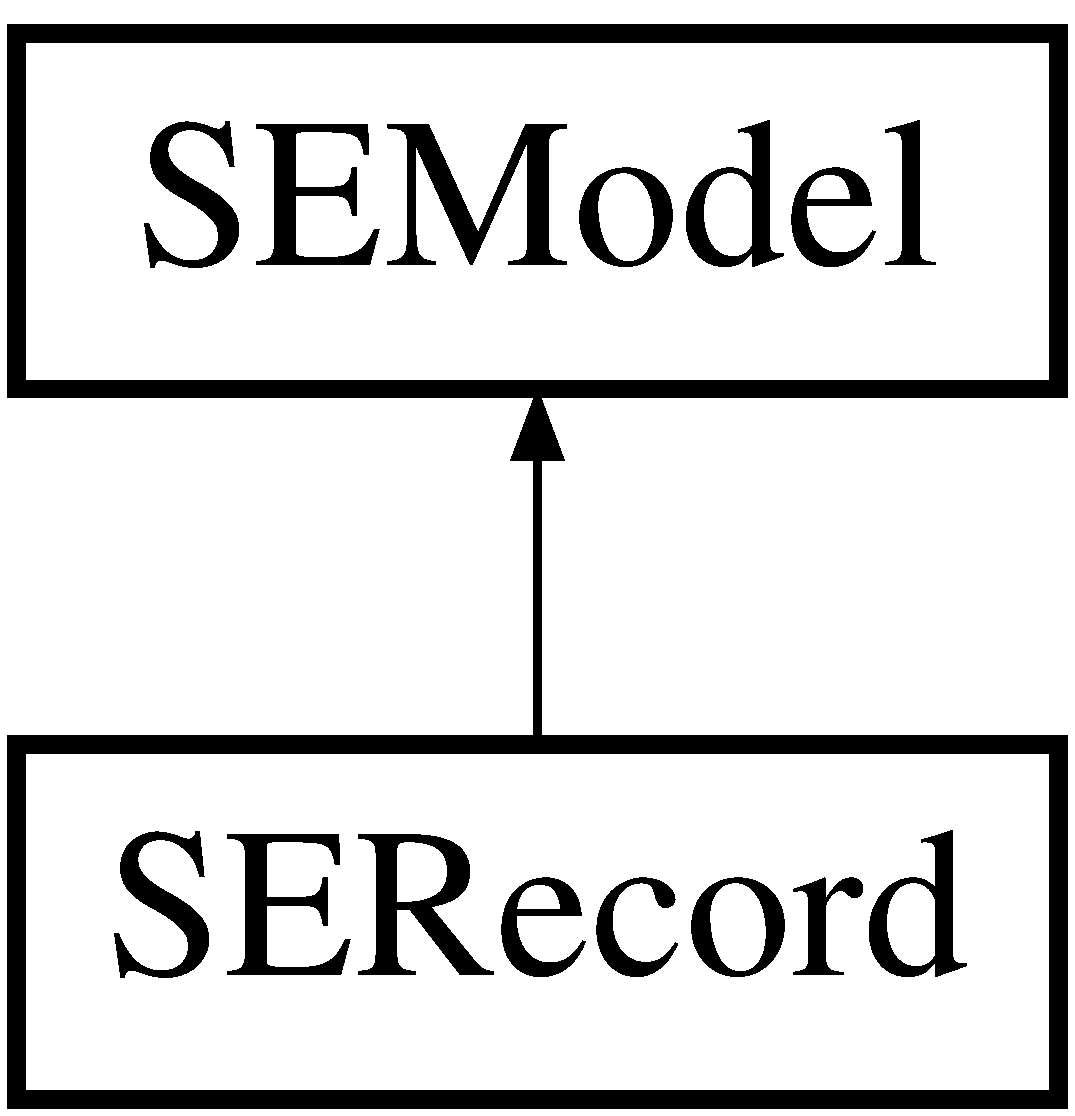
\includegraphics[height=2.000000cm]{interface_s_e_record}
\end{center}
\end{figure}
\subsection*{Properties}
\begin{DoxyCompactItemize}
\item 
\hyperlink{interface_s_e_project}{S\-E\-Project} $\ast$ \hyperlink{interface_s_e_record_a6051966cb1a3a4f0dcf0e3963fc9d129}{project}
\item 
\hyperlink{interface_s_e_sound}{S\-E\-Sound} $\ast$ \hyperlink{interface_s_e_record_a5fe4fce40492a08dafb34f659ff35ceb}{sound}
\item 
N\-S\-String $\ast$ \hyperlink{interface_s_e_record_aaf616132fe7f963e0c791e00b12e6f92}{sound\-Path}
\item 
\hyperlink{struct_s_r_sound_range}{S\-R\-Sound\-Range} \hyperlink{interface_s_e_record_ac529abfcc62ecfb7123a8ecae4431822}{time\-Range}
\item 
C\-M\-Time\-Range \hyperlink{interface_s_e_record_ad11719c2813141c0a4fc23da025382f0}{asset\-Time\-Range}
\end{DoxyCompactItemize}


\subsection{Property Documentation}
\hypertarget{interface_s_e_record_ad11719c2813141c0a4fc23da025382f0}{\index{S\-E\-Record@{S\-E\-Record}!asset\-Time\-Range@{asset\-Time\-Range}}
\index{asset\-Time\-Range@{asset\-Time\-Range}!SERecord@{S\-E\-Record}}
\subsubsection[{asset\-Time\-Range}]{\setlength{\rightskip}{0pt plus 5cm}-\/ (C\-M\-Time\-Range) asset\-Time\-Range\hspace{0.3cm}{\ttfamily [read]}, {\ttfamily [nonatomic]}, {\ttfamily [assign]}}}\label{interface_s_e_record_ad11719c2813141c0a4fc23da025382f0}
\hypertarget{interface_s_e_record_a6051966cb1a3a4f0dcf0e3963fc9d129}{\index{S\-E\-Record@{S\-E\-Record}!project@{project}}
\index{project@{project}!SERecord@{S\-E\-Record}}
\subsubsection[{project}]{\setlength{\rightskip}{0pt plus 5cm}-\/ ({\bf S\-E\-Project}$\ast$) project\hspace{0.3cm}{\ttfamily [read]}, {\ttfamily [write]}, {\ttfamily [nonatomic]}, {\ttfamily [weak]}}}\label{interface_s_e_record_a6051966cb1a3a4f0dcf0e3963fc9d129}
\hypertarget{interface_s_e_record_a5fe4fce40492a08dafb34f659ff35ceb}{\index{S\-E\-Record@{S\-E\-Record}!sound@{sound}}
\index{sound@{sound}!SERecord@{S\-E\-Record}}
\subsubsection[{sound}]{\setlength{\rightskip}{0pt plus 5cm}-\/ ({\bf S\-E\-Sound} $\ast$) sound\hspace{0.3cm}{\ttfamily [read]}, {\ttfamily [nonatomic]}, {\ttfamily [assign]}}}\label{interface_s_e_record_a5fe4fce40492a08dafb34f659ff35ceb}
\hypertarget{interface_s_e_record_aaf616132fe7f963e0c791e00b12e6f92}{\index{S\-E\-Record@{S\-E\-Record}!sound\-Path@{sound\-Path}}
\index{sound\-Path@{sound\-Path}!SERecord@{S\-E\-Record}}
\subsubsection[{sound\-Path}]{\setlength{\rightskip}{0pt plus 5cm}-\/ (N\-S\-String$\ast$) sound\-Path\hspace{0.3cm}{\ttfamily [read]}, {\ttfamily [write]}, {\ttfamily [nonatomic]}, {\ttfamily [strong]}}}\label{interface_s_e_record_aaf616132fe7f963e0c791e00b12e6f92}
\hypertarget{interface_s_e_record_ac529abfcc62ecfb7123a8ecae4431822}{\index{S\-E\-Record@{S\-E\-Record}!time\-Range@{time\-Range}}
\index{time\-Range@{time\-Range}!SERecord@{S\-E\-Record}}
\subsubsection[{time\-Range}]{\setlength{\rightskip}{0pt plus 5cm}-\/ ({\bf S\-R\-Sound\-Range}) time\-Range\hspace{0.3cm}{\ttfamily [read]}, {\ttfamily [write]}, {\ttfamily [nonatomic]}, {\ttfamily [assign]}}}\label{interface_s_e_record_ac529abfcc62ecfb7123a8ecae4431822}


The documentation for this class was generated from the following files\-:\begin{DoxyCompactItemize}
\item 
Sound\-Recorder/\-Classes/\-Core/\-Sound\-Editor/\hyperlink{_s_e_record_8h}{S\-E\-Record.\-h}\item 
Sound\-Recorder/\-Classes/\-Core/\-Sound\-Editor/\hyperlink{_s_e_record_8m}{S\-E\-Record.\-m}\end{DoxyCompactItemize}

\hypertarget{interface_s_e_record_audio_stream}{\section{S\-E\-Record\-Audio\-Stream Class Reference}
\label{interface_s_e_record_audio_stream}\index{S\-E\-Record\-Audio\-Stream@{S\-E\-Record\-Audio\-Stream}}
}


{\ttfamily \#import $<$S\-E\-Record\-Audio\-Stream.\-h$>$}



Inheritance diagram for S\-E\-Record\-Audio\-Stream\-:


Collaboration diagram for S\-E\-Record\-Audio\-Stream\-:
\subsection*{Instance Methods}
\begin{DoxyCompactItemize}
\item 
(id) -\/ \hyperlink{interface_s_e_record_audio_stream_a92c7ab157006ec7f599b742512173417}{init\-With\-Record\-:}
\item 
(void) -\/ \hyperlink{interface_s_e_record_audio_stream_afa78c4835ce4e83bfca38800faed0f33}{start\-Recording}
\item 
(void) -\/ \hyperlink{interface_s_e_record_audio_stream_a10e91ee60958add80d70acbf6741b2db}{stop\-Recording}
\end{DoxyCompactItemize}
\subsection*{Properties}
\begin{DoxyCompactItemize}
\item 
id$<$ S\-E\-Record\-Audio\-Stream\-Delegate $>$ \hyperlink{interface_s_e_record_audio_stream_a63ed0771101a0265b303e0ae90a4258a}{delegate}
\item 
S\-R\-Record $\ast$ \hyperlink{interface_s_e_record_audio_stream_a7f9b00906c871fef706dd86b29044185}{record}
\end{DoxyCompactItemize}


\subsection{Method Documentation}
\hypertarget{interface_s_e_record_audio_stream_a92c7ab157006ec7f599b742512173417}{\index{S\-E\-Record\-Audio\-Stream@{S\-E\-Record\-Audio\-Stream}!init\-With\-Record\-:@{init\-With\-Record\-:}}
\index{init\-With\-Record\-:@{init\-With\-Record\-:}!SERecordAudioStream@{S\-E\-Record\-Audio\-Stream}}
\subsubsection[{init\-With\-Record\-:}]{\setlength{\rightskip}{0pt plus 5cm}-\/ (id) init\-With\-Record\-: 
\begin{DoxyParamCaption}
\item[{(S\-R\-Record$\ast$)}]{record}
\end{DoxyParamCaption}
}}\label{interface_s_e_record_audio_stream_a92c7ab157006ec7f599b742512173417}
Initialize stream with record 

Here is the call graph for this function\-:


\hypertarget{interface_s_e_record_audio_stream_afa78c4835ce4e83bfca38800faed0f33}{\index{S\-E\-Record\-Audio\-Stream@{S\-E\-Record\-Audio\-Stream}!start\-Recording@{start\-Recording}}
\index{start\-Recording@{start\-Recording}!SERecordAudioStream@{S\-E\-Record\-Audio\-Stream}}
\subsubsection[{start\-Recording}]{\setlength{\rightskip}{0pt plus 5cm}-\/ (void) start\-Recording 
\begin{DoxyParamCaption}
{}
\end{DoxyParamCaption}
}}\label{interface_s_e_record_audio_stream_afa78c4835ce4e83bfca38800faed0f33}
Start recording sound \hypertarget{interface_s_e_record_audio_stream_a10e91ee60958add80d70acbf6741b2db}{\index{S\-E\-Record\-Audio\-Stream@{S\-E\-Record\-Audio\-Stream}!stop\-Recording@{stop\-Recording}}
\index{stop\-Recording@{stop\-Recording}!SERecordAudioStream@{S\-E\-Record\-Audio\-Stream}}
\subsubsection[{stop\-Recording}]{\setlength{\rightskip}{0pt plus 5cm}-\/ (void) stop\-Recording 
\begin{DoxyParamCaption}
{}
\end{DoxyParamCaption}
}}\label{interface_s_e_record_audio_stream_a10e91ee60958add80d70acbf6741b2db}
Stop recording sound 

\subsection{Property Documentation}
\hypertarget{interface_s_e_record_audio_stream_a63ed0771101a0265b303e0ae90a4258a}{\index{S\-E\-Record\-Audio\-Stream@{S\-E\-Record\-Audio\-Stream}!delegate@{delegate}}
\index{delegate@{delegate}!SERecordAudioStream@{S\-E\-Record\-Audio\-Stream}}
\subsubsection[{delegate}]{\setlength{\rightskip}{0pt plus 5cm}-\/ (id$<$S\-E\-Record\-Audio\-Stream\-Delegate$>$) delegate\hspace{0.3cm}{\ttfamily [read]}, {\ttfamily [write]}, {\ttfamily [nonatomic]}, {\ttfamily [weak]}}}\label{interface_s_e_record_audio_stream_a63ed0771101a0265b303e0ae90a4258a}
\hypertarget{interface_s_e_record_audio_stream_a7f9b00906c871fef706dd86b29044185}{\index{S\-E\-Record\-Audio\-Stream@{S\-E\-Record\-Audio\-Stream}!record@{record}}
\index{record@{record}!SERecordAudioStream@{S\-E\-Record\-Audio\-Stream}}
\subsubsection[{record}]{\setlength{\rightskip}{0pt plus 5cm}-\/ (S\-R\-Record$\ast$) record\hspace{0.3cm}{\ttfamily [read]}, {\ttfamily [nonatomic]}, {\ttfamily [assign]}}}\label{interface_s_e_record_audio_stream_a7f9b00906c871fef706dd86b29044185}
Pointer to record 

The documentation for this class was generated from the following files\-:\begin{DoxyCompactItemize}
\item 
/\-Users/igor/\-Develop/\-Develop\-Git/\-Davacon/i\-Phone/\-Sound\-Recorder/\-Classes/\-Core/\-Sound\-Editor/\hyperlink{_s_e_record_audio_stream_8h}{S\-E\-Record\-Audio\-Stream.\-h}\item 
/\-Users/igor/\-Develop/\-Develop\-Git/\-Davacon/i\-Phone/\-Sound\-Recorder/\-Classes/\-Core/\-Sound\-Editor/\hyperlink{_s_e_record_audio_stream_8m}{S\-E\-Record\-Audio\-Stream.\-m}\end{DoxyCompactItemize}

\hypertarget{protocol_s_e_record_audio_stream_delegate-p}{\section{$<$S\-E\-Record\-Audio\-Stream\-Delegate$>$ Protocol Reference}
\label{protocol_s_e_record_audio_stream_delegate-p}\index{$<$\-S\-E\-Record\-Audio\-Stream\-Delegate$>$@{$<$\-S\-E\-Record\-Audio\-Stream\-Delegate$>$}}
}


{\ttfamily \#import $<$S\-E\-Record\-Audio\-Stream.\-h$>$}

Inheritance diagram for $<$S\-E\-Record\-Audio\-Stream\-Delegate$>$\-:\begin{figure}[H]
\begin{center}
\leavevmode
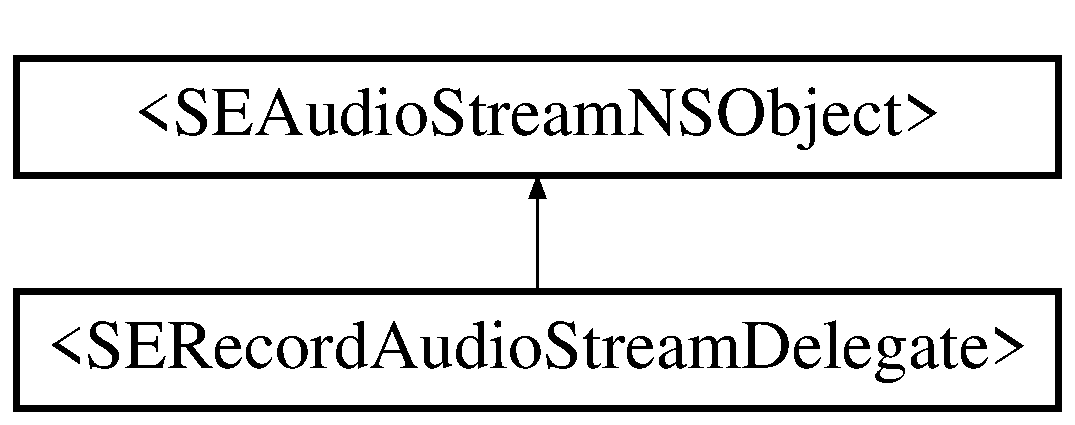
\includegraphics[height=2.000000cm]{protocol_s_e_record_audio_stream_delegate-p}
\end{center}
\end{figure}
\subsection*{Instance Methods}
\begin{DoxyCompactItemize}
\item 
(void) -\/ \hyperlink{protocol_s_e_record_audio_stream_delegate-p_ad9a82cf4916f8d3dc0450d7904244272}{record\-Audio\-Stream\-Did\-Start\-Recording\-:}
\item 
(void) -\/ \hyperlink{protocol_s_e_record_audio_stream_delegate-p_a6f989682abec086abcf3df35aa465b64}{record\-Audio\-Stream\-:did\-Update\-With\-Duration\-:}
\item 
(void) -\/ \hyperlink{protocol_s_e_record_audio_stream_delegate-p_adfc35cb87b18e6b20e2e02f8894defa8}{record\-Audio\-Stream\-Did\-Finish\-Recording\-:}
\end{DoxyCompactItemize}


\subsection{Method Documentation}
\hypertarget{protocol_s_e_record_audio_stream_delegate-p_a6f989682abec086abcf3df35aa465b64}{\index{S\-E\-Record\-Audio\-Stream\-Delegate-\/p@{S\-E\-Record\-Audio\-Stream\-Delegate-\/p}!record\-Audio\-Stream\-:did\-Update\-With\-Duration\-:@{record\-Audio\-Stream\-:did\-Update\-With\-Duration\-:}}
\index{record\-Audio\-Stream\-:did\-Update\-With\-Duration\-:@{record\-Audio\-Stream\-:did\-Update\-With\-Duration\-:}!SERecordAudioStreamDelegate-p@{S\-E\-Record\-Audio\-Stream\-Delegate-\/p}}
\subsubsection[{record\-Audio\-Stream\-:did\-Update\-With\-Duration\-:}]{\setlength{\rightskip}{0pt plus 5cm}-\/ (void) record\-Audio\-Stream\-: 
\begin{DoxyParamCaption}
\item[{({\bf S\-E\-Record\-Audio\-Stream} $\ast$)}]{stream}
\item[{didUpdateWithDuration:(N\-S\-Time\-Interval)}]{duration}
\end{DoxyParamCaption}
}}\label{protocol_s_e_record_audio_stream_delegate-p_a6f989682abec086abcf3df35aa465b64}
Notification for update recording info \hypertarget{protocol_s_e_record_audio_stream_delegate-p_adfc35cb87b18e6b20e2e02f8894defa8}{\index{S\-E\-Record\-Audio\-Stream\-Delegate-\/p@{S\-E\-Record\-Audio\-Stream\-Delegate-\/p}!record\-Audio\-Stream\-Did\-Finish\-Recording\-:@{record\-Audio\-Stream\-Did\-Finish\-Recording\-:}}
\index{record\-Audio\-Stream\-Did\-Finish\-Recording\-:@{record\-Audio\-Stream\-Did\-Finish\-Recording\-:}!SERecordAudioStreamDelegate-p@{S\-E\-Record\-Audio\-Stream\-Delegate-\/p}}
\subsubsection[{record\-Audio\-Stream\-Did\-Finish\-Recording\-:}]{\setlength{\rightskip}{0pt plus 5cm}-\/ (void) record\-Audio\-Stream\-Did\-Finish\-Recording\-: 
\begin{DoxyParamCaption}
\item[{({\bf S\-E\-Record\-Audio\-Stream} $\ast$)}]{stream}
\end{DoxyParamCaption}
}}\label{protocol_s_e_record_audio_stream_delegate-p_adfc35cb87b18e6b20e2e02f8894defa8}
Notification for end recording \hypertarget{protocol_s_e_record_audio_stream_delegate-p_ad9a82cf4916f8d3dc0450d7904244272}{\index{S\-E\-Record\-Audio\-Stream\-Delegate-\/p@{S\-E\-Record\-Audio\-Stream\-Delegate-\/p}!record\-Audio\-Stream\-Did\-Start\-Recording\-:@{record\-Audio\-Stream\-Did\-Start\-Recording\-:}}
\index{record\-Audio\-Stream\-Did\-Start\-Recording\-:@{record\-Audio\-Stream\-Did\-Start\-Recording\-:}!SERecordAudioStreamDelegate-p@{S\-E\-Record\-Audio\-Stream\-Delegate-\/p}}
\subsubsection[{record\-Audio\-Stream\-Did\-Start\-Recording\-:}]{\setlength{\rightskip}{0pt plus 5cm}-\/ (void) record\-Audio\-Stream\-Did\-Start\-Recording\-: 
\begin{DoxyParamCaption}
\item[{({\bf S\-E\-Record\-Audio\-Stream} $\ast$)}]{stream}
\end{DoxyParamCaption}
}}\label{protocol_s_e_record_audio_stream_delegate-p_ad9a82cf4916f8d3dc0450d7904244272}
Notification for begin recording 

The documentation for this protocol was generated from the following file\-:\begin{DoxyCompactItemize}
\item 
/\-Users/igor/\-Develop/\-Develop\-Git/\-Davacon/i\-Phone/\-Sound\-Recorder/\-Classes/\-Core/\-Sound\-Editor/\hyperlink{_s_e_record_audio_stream_8h}{S\-E\-Record\-Audio\-Stream.\-h}\end{DoxyCompactItemize}

\hypertarget{struct_s_e_record_sound_range}{\section{S\-E\-Record\-Sound\-Range Struct Reference}
\label{struct_s_e_record_sound_range}\index{S\-E\-Record\-Sound\-Range@{S\-E\-Record\-Sound\-Range}}
}


{\ttfamily \#import $<$S\-E\-Record.\-h$>$}

\subsection*{Protected Attributes}
\begin{DoxyCompactItemize}
\item 
N\-S\-Time\-Interval \hyperlink{struct_s_e_record_sound_range_a68e4b0862e4a25d22219776f0a9d4bc9}{start}
\item 
N\-S\-Time\-Interval \hyperlink{struct_s_e_record_sound_range_a9c2cd7852875423d8bde9118fd62f85b}{duration}
\end{DoxyCompactItemize}


\subsection{Member Data Documentation}
\hypertarget{struct_s_e_record_sound_range_a9c2cd7852875423d8bde9118fd62f85b}{\index{S\-E\-Record\-Sound\-Range@{S\-E\-Record\-Sound\-Range}!duration@{duration}}
\index{duration@{duration}!SERecordSoundRange@{S\-E\-Record\-Sound\-Range}}
\subsubsection[{duration}]{\setlength{\rightskip}{0pt plus 5cm}-\/ (N\-S\-Time\-Interval) duration\hspace{0.3cm}{\ttfamily [protected]}}}\label{struct_s_e_record_sound_range_a9c2cd7852875423d8bde9118fd62f85b}
Sound start position \hypertarget{struct_s_e_record_sound_range_a68e4b0862e4a25d22219776f0a9d4bc9}{\index{S\-E\-Record\-Sound\-Range@{S\-E\-Record\-Sound\-Range}!start@{start}}
\index{start@{start}!SERecordSoundRange@{S\-E\-Record\-Sound\-Range}}
\subsubsection[{start}]{\setlength{\rightskip}{0pt plus 5cm}-\/ (N\-S\-Time\-Interval) start\hspace{0.3cm}{\ttfamily [protected]}}}\label{struct_s_e_record_sound_range_a68e4b0862e4a25d22219776f0a9d4bc9}


The documentation for this struct was generated from the following file\-:\begin{DoxyCompactItemize}
\item 
/\-Users/igor/\-Develop/\-Develop\-Git/\-Davacon/i\-Phone/\-Sound\-Recorder/\-Classes/\-Core/\-Sound\-Editor/\hyperlink{_s_e_record_8h}{S\-E\-Record.\-h}\end{DoxyCompactItemize}

\hypertarget{interface_s_e_speex_a_c_m_audio_stream}{\section{S\-E\-Speex\-A\-C\-M\-Audio\-Stream Class Reference}
\label{interface_s_e_speex_a_c_m_audio_stream}\index{S\-E\-Speex\-A\-C\-M\-Audio\-Stream@{S\-E\-Speex\-A\-C\-M\-Audio\-Stream}}
}


{\ttfamily \#import $<$S\-E\-Speex\-A\-C\-M\-Audio\-Stream.\-h$>$}

Inheritance diagram for S\-E\-Speex\-A\-C\-M\-Audio\-Stream\-:\begin{figure}[H]
\begin{center}
\leavevmode
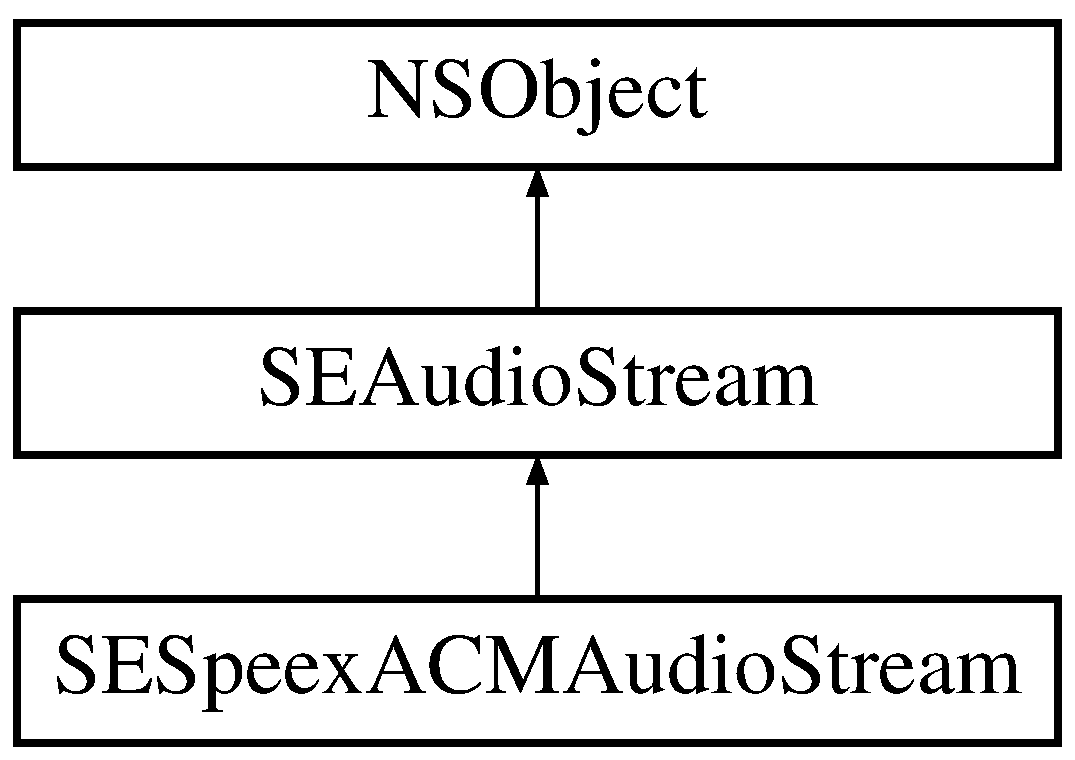
\includegraphics[height=3.000000cm]{interface_s_e_speex_a_c_m_audio_stream}
\end{center}
\end{figure}
\subsection*{Additional Inherited Members}


The documentation for this class was generated from the following file\-:\begin{DoxyCompactItemize}
\item 
/\-Users/igor/\-Develop/\-Develop\-Git/\-Davacon/i\-Phone/\-Sound\-Recorder/\-Classes/\-Core/\-Sound\-Editor/\hyperlink{_s_e_speex_a_c_m_audio_stream_8h}{S\-E\-Speex\-A\-C\-M\-Audio\-Stream.\-h}\end{DoxyCompactItemize}

\chapter{File Documentation}
\hypertarget{_s_e_audio_stream_8h}{\section{Sound\-Recorder/\-Classes/\-Core/\-Sound\-Editor/\-S\-E\-Audio\-Stream.h File Reference}
\label{_s_e_audio_stream_8h}\index{Sound\-Recorder/\-Classes/\-Core/\-Sound\-Editor/\-S\-E\-Audio\-Stream.\-h@{Sound\-Recorder/\-Classes/\-Core/\-Sound\-Editor/\-S\-E\-Audio\-Stream.\-h}}
}
{\ttfamily \#import $<$Audio\-Toolbox/\-Audio\-Toolbox.\-h$>$}\\*
\subsection*{Classes}
\begin{DoxyCompactItemize}
\item 
class \hyperlink{interface_s_e_audio_stream}{S\-E\-Audio\-Stream}
\item 
category \hyperlink{category_s_e_audio_stream_07_write_08}{S\-E\-Audio\-Stream(\-Write)}
\item 
category \hyperlink{category_s_e_audio_stream_07_read_08}{S\-E\-Audio\-Stream(\-Read)}
\end{DoxyCompactItemize}

\hypertarget{_s_e_audio_stream_8m}{\section{Sound\-Recorder/\-Classes/\-Core/\-Sound\-Editor/\-S\-E\-Audio\-Stream.m File Reference}
\label{_s_e_audio_stream_8m}\index{Sound\-Recorder/\-Classes/\-Core/\-Sound\-Editor/\-S\-E\-Audio\-Stream.\-m@{Sound\-Recorder/\-Classes/\-Core/\-Sound\-Editor/\-S\-E\-Audio\-Stream.\-m}}
}
{\ttfamily \#import \char`\"{}S\-E\-Audio\-Stream.\-h\char`\"{}}\\*

\hypertarget{_s_e_audio_stream_player_8h}{\section{/\-Users/igor/\-Develop/\-Develop\-Git/\-Davacon/i\-Phone/\-Sound\-Recorder/\-Classes/\-Core/\-Sound\-Editor/\-S\-E\-Audio\-Stream\-Player.h File Reference}
\label{_s_e_audio_stream_player_8h}\index{/\-Users/igor/\-Develop/\-Develop\-Git/\-Davacon/i\-Phone/\-Sound\-Recorder/\-Classes/\-Core/\-Sound\-Editor/\-S\-E\-Audio\-Stream\-Player.\-h@{/\-Users/igor/\-Develop/\-Develop\-Git/\-Davacon/i\-Phone/\-Sound\-Recorder/\-Classes/\-Core/\-Sound\-Editor/\-S\-E\-Audio\-Stream\-Player.\-h}}
}
{\ttfamily \#import $<$Audio\-Toolbox/\-Audio\-Toolbox.\-h$>$}\\*
\subsection*{Classes}
\begin{DoxyCompactItemize}
\item 
class \hyperlink{interface_s_e_audio_stream_player}{S\-E\-Audio\-Stream\-Player}
\item 
protocol \hyperlink{protocol_s_e_audio_stream_player_delegate-p}{$<$\-S\-E\-Audio\-Stream\-Player\-Delegate$>$}
\end{DoxyCompactItemize}

\hypertarget{_s_e_audio_stream_player_8m}{\section{/\-Users/igor/\-Develop/\-Develop\-Git/\-Davacon/i\-Phone/\-Sound\-Recorder/\-Classes/\-Core/\-Sound\-Editor/\-S\-E\-Audio\-Stream\-Player.m File Reference}
\label{_s_e_audio_stream_player_8m}\index{/\-Users/igor/\-Develop/\-Develop\-Git/\-Davacon/i\-Phone/\-Sound\-Recorder/\-Classes/\-Core/\-Sound\-Editor/\-S\-E\-Audio\-Stream\-Player.\-m@{/\-Users/igor/\-Develop/\-Develop\-Git/\-Davacon/i\-Phone/\-Sound\-Recorder/\-Classes/\-Core/\-Sound\-Editor/\-S\-E\-Audio\-Stream\-Player.\-m}}
}
{\ttfamily \#import \char`\"{}S\-E\-Audio\-Stream\-Player.\-h\char`\"{}}\\*

\hypertarget{_s_e_project_8h}{\section{/\-Users/igor/\-Develop/\-Develop\-Git/\-Davacon/i\-Phone/\-Sound\-Recorder/\-Classes/\-Core/\-Sound\-Editor/\-S\-E\-Project.h File Reference}
\label{_s_e_project_8h}\index{/\-Users/igor/\-Develop/\-Develop\-Git/\-Davacon/i\-Phone/\-Sound\-Recorder/\-Classes/\-Core/\-Sound\-Editor/\-S\-E\-Project.\-h@{/\-Users/igor/\-Develop/\-Develop\-Git/\-Davacon/i\-Phone/\-Sound\-Recorder/\-Classes/\-Core/\-Sound\-Editor/\-S\-E\-Project.\-h}}
}
{\ttfamily \#import \char`\"{}S\-E\-Model.\-h\char`\"{}}\\*
{\ttfamily \#import \char`\"{}S\-E\-Audio\-Stream\-Player.\-h\char`\"{}}\\*
{\ttfamily \#import \char`\"{}S\-E\-Record.\-h\char`\"{}}\\*
\subsection*{Classes}
\begin{DoxyCompactItemize}
\item 
class \hyperlink{interface_s_e_project}{S\-E\-Project}
\end{DoxyCompactItemize}

\hypertarget{_s_e_project_8m}{\section{/\-Users/igor/\-Develop/\-Develop\-Git/\-Davacon/i\-Phone/\-Sound\-Recorder/\-Classes/\-Core/\-Sound\-Editor/\-S\-E\-Project.m File Reference}
\label{_s_e_project_8m}\index{/\-Users/igor/\-Develop/\-Develop\-Git/\-Davacon/i\-Phone/\-Sound\-Recorder/\-Classes/\-Core/\-Sound\-Editor/\-S\-E\-Project.\-m@{/\-Users/igor/\-Develop/\-Develop\-Git/\-Davacon/i\-Phone/\-Sound\-Recorder/\-Classes/\-Core/\-Sound\-Editor/\-S\-E\-Project.\-m}}
}
{\ttfamily \#import \char`\"{}S\-E\-Project.\-h\char`\"{}}\\*
{\ttfamily \#import \char`\"{}S\-E\-Record.\-h\char`\"{}}\\*
{\ttfamily \#import \char`\"{}S\-E\-Project+\-Internal.\-h\char`\"{}}\\*

\hypertarget{_s_e_project_audio_stream_8h}{\section{/\-Users/igor/\-Develop/\-Develop\-Git/\-Davacon/i\-Phone/\-Sound\-Recorder/\-Classes/\-Core/\-Sound\-Editor/\-S\-E\-Project\-Audio\-Stream.h File Reference}
\label{_s_e_project_audio_stream_8h}\index{/\-Users/igor/\-Develop/\-Develop\-Git/\-Davacon/i\-Phone/\-Sound\-Recorder/\-Classes/\-Core/\-Sound\-Editor/\-S\-E\-Project\-Audio\-Stream.\-h@{/\-Users/igor/\-Develop/\-Develop\-Git/\-Davacon/i\-Phone/\-Sound\-Recorder/\-Classes/\-Core/\-Sound\-Editor/\-S\-E\-Project\-Audio\-Stream.\-h}}
}
{\ttfamily \#import \char`\"{}S\-E\-Audio\-Stream.\-h\char`\"{}}\\*
Include dependency graph for S\-E\-Project\-Audio\-Stream.\-h\-:
This graph shows which files directly or indirectly include this file\-:
\subsection*{Classes}
\begin{DoxyCompactItemize}
\item 
class \hyperlink{interface_s_e_project_audio_stream}{S\-E\-Project\-Audio\-Stream}
\end{DoxyCompactItemize}

\hypertarget{_s_e_project_audio_stream_8m}{\section{/\-Users/igor/\-Develop/\-Develop\-Git/\-Davacon/i\-Phone/\-Sound\-Recorder/\-Classes/\-Core/\-Sound\-Editor/\-S\-E\-Project\-Audio\-Stream.m File Reference}
\label{_s_e_project_audio_stream_8m}\index{/\-Users/igor/\-Develop/\-Develop\-Git/\-Davacon/i\-Phone/\-Sound\-Recorder/\-Classes/\-Core/\-Sound\-Editor/\-S\-E\-Project\-Audio\-Stream.\-m@{/\-Users/igor/\-Develop/\-Develop\-Git/\-Davacon/i\-Phone/\-Sound\-Recorder/\-Classes/\-Core/\-Sound\-Editor/\-S\-E\-Project\-Audio\-Stream.\-m}}
}
{\ttfamily \#import \char`\"{}S\-E\-Project\-Audio\-Stream.\-h\char`\"{}}\\*
Include dependency graph for S\-E\-Project\-Audio\-Stream.\-m\-:

\hypertarget{_s_e_record_8h}{\section{Sound\-Recorder/\-Classes/\-Core/\-Sound\-Editor/\-S\-E\-Record.h File Reference}
\label{_s_e_record_8h}\index{Sound\-Recorder/\-Classes/\-Core/\-Sound\-Editor/\-S\-E\-Record.\-h@{Sound\-Recorder/\-Classes/\-Core/\-Sound\-Editor/\-S\-E\-Record.\-h}}
}
{\ttfamily \#import \char`\"{}S\-R\-Model.\-h\char`\"{}}\\*
{\ttfamily \#import \char`\"{}S\-E\-Sound.\-h\char`\"{}}\\*
{\ttfamily \#import $<$A\-V\-Foundation/\-A\-V\-Foundation.\-h$>$}\\*
\subsection*{Classes}
\begin{DoxyCompactItemize}
\item 
class \hyperlink{interface_s_e_record}{S\-E\-Record}
\end{DoxyCompactItemize}

\hypertarget{_s_e_record_8m}{\section{/\-Users/igor/\-Develop/\-Develop\-Git/\-Davacon/i\-Phone/\-Sound\-Recorder/\-Classes/\-Core/\-Sound\-Editor/\-S\-E\-Record.m File Reference}
\label{_s_e_record_8m}\index{/\-Users/igor/\-Develop/\-Develop\-Git/\-Davacon/i\-Phone/\-Sound\-Recorder/\-Classes/\-Core/\-Sound\-Editor/\-S\-E\-Record.\-m@{/\-Users/igor/\-Develop/\-Develop\-Git/\-Davacon/i\-Phone/\-Sound\-Recorder/\-Classes/\-Core/\-Sound\-Editor/\-S\-E\-Record.\-m}}
}
{\ttfamily \#import \char`\"{}S\-E\-Record.\-h\char`\"{}}\\*
Include dependency graph for S\-E\-Record.\-m\-:

\hypertarget{_s_e_record_audio_stream_8h}{\section{/\-Users/igor/\-Develop/\-Develop\-Git/\-Davacon/i\-Phone/\-Sound\-Recorder/\-Classes/\-Core/\-Sound\-Editor/\-S\-E\-Record\-Audio\-Stream.h File Reference}
\label{_s_e_record_audio_stream_8h}\index{/\-Users/igor/\-Develop/\-Develop\-Git/\-Davacon/i\-Phone/\-Sound\-Recorder/\-Classes/\-Core/\-Sound\-Editor/\-S\-E\-Record\-Audio\-Stream.\-h@{/\-Users/igor/\-Develop/\-Develop\-Git/\-Davacon/i\-Phone/\-Sound\-Recorder/\-Classes/\-Core/\-Sound\-Editor/\-S\-E\-Record\-Audio\-Stream.\-h}}
}
{\ttfamily \#import \char`\"{}S\-E\-Audio\-Stream.\-h\char`\"{}}\\*
\subsection*{Classes}
\begin{DoxyCompactItemize}
\item 
class \hyperlink{interface_s_e_record_audio_stream}{S\-E\-Record\-Audio\-Stream}
\item 
protocol \hyperlink{protocol_s_e_record_audio_stream_delegate-p}{$<$\-S\-E\-Record\-Audio\-Stream\-Delegate$>$}
\end{DoxyCompactItemize}

\hypertarget{_s_e_record_audio_stream_8m}{\section{/\-Users/igor/\-Develop/\-Develop\-Git/\-Davacon/i\-Phone/\-Sound\-Recorder/\-Classes/\-Core/\-Sound\-Editor/\-S\-E\-Record\-Audio\-Stream.m File Reference}
\label{_s_e_record_audio_stream_8m}\index{/\-Users/igor/\-Develop/\-Develop\-Git/\-Davacon/i\-Phone/\-Sound\-Recorder/\-Classes/\-Core/\-Sound\-Editor/\-S\-E\-Record\-Audio\-Stream.\-m@{/\-Users/igor/\-Develop/\-Develop\-Git/\-Davacon/i\-Phone/\-Sound\-Recorder/\-Classes/\-Core/\-Sound\-Editor/\-S\-E\-Record\-Audio\-Stream.\-m}}
}
{\ttfamily \#import \char`\"{}S\-E\-Record\-Audio\-Stream.\-h\char`\"{}}\\*

\hypertarget{_s_e_speex_a_c_m_audio_stream_8h}{\section{/\-Users/igor/\-Develop/\-Develop\-Git/\-Davacon/i\-Phone/\-Sound\-Recorder/\-Classes/\-Core/\-Sound\-Editor/\-S\-E\-Speex\-A\-C\-M\-Audio\-Stream.h File Reference}
\label{_s_e_speex_a_c_m_audio_stream_8h}\index{/\-Users/igor/\-Develop/\-Develop\-Git/\-Davacon/i\-Phone/\-Sound\-Recorder/\-Classes/\-Core/\-Sound\-Editor/\-S\-E\-Speex\-A\-C\-M\-Audio\-Stream.\-h@{/\-Users/igor/\-Develop/\-Develop\-Git/\-Davacon/i\-Phone/\-Sound\-Recorder/\-Classes/\-Core/\-Sound\-Editor/\-S\-E\-Speex\-A\-C\-M\-Audio\-Stream.\-h}}
}
{\ttfamily \#import \char`\"{}S\-E\-Audio\-Stream.\-h\char`\"{}}\\*
\subsection*{Classes}
\begin{DoxyCompactItemize}
\item 
class \hyperlink{interface_s_e_speex_a_c_m_audio_stream}{S\-E\-Speex\-A\-C\-M\-Audio\-Stream}
\end{DoxyCompactItemize}

\hypertarget{_s_e_speex_a_c_m_audio_stream_8m}{\section{/\-Users/igor/\-Develop/\-Develop\-Git/\-Davacon/i\-Phone/\-Sound\-Recorder/\-Classes/\-Core/\-Sound\-Editor/\-S\-E\-Speex\-A\-C\-M\-Audio\-Stream.m File Reference}
\label{_s_e_speex_a_c_m_audio_stream_8m}\index{/\-Users/igor/\-Develop/\-Develop\-Git/\-Davacon/i\-Phone/\-Sound\-Recorder/\-Classes/\-Core/\-Sound\-Editor/\-S\-E\-Speex\-A\-C\-M\-Audio\-Stream.\-m@{/\-Users/igor/\-Develop/\-Develop\-Git/\-Davacon/i\-Phone/\-Sound\-Recorder/\-Classes/\-Core/\-Sound\-Editor/\-S\-E\-Speex\-A\-C\-M\-Audio\-Stream.\-m}}
}
{\ttfamily \#import \char`\"{}S\-E\-Speex\-A\-C\-M\-Audio\-Stream.\-h\char`\"{}}\\*
{\ttfamily \#import \char`\"{}S\-E\-Speex\-A\-C\-M\-Wrapper.\-h\char`\"{}}\\*
{\ttfamily \#import \char`\"{}S\-E\-Audio\-Stream+\-Internal.\-h\char`\"{}}\\*

%--- End generated contents ---

% Index
\newpage
\phantomsection
\addcontentsline{toc}{chapter}{Index}
\printindex

\end{document}
